\section{Pairs, Linkages, and Configurations}

\begin{frame}
	\frametitle{Outline}
	\begin{tcolorbox}[coltitle=white!80,colframe=blue!85,split=.2,title=Mechanism Components]
		Kinematic geometry. Mechanisms.
		\tcblower
		Joints: Joint closure; Pairs; Couplings.
		\vspace{.2cm}
		\newline
		Lower pairs and linkages; Higher and lower pairs.
		\vspace{.2cm}
		\newline
		Motions: Planar and spherical motions.
		\vspace{.2cm}
		\newline
		Synthesis: Type-, number-, and size-syntheses.
	\end{tcolorbox}
\end{frame}

\subsection{Mechanics}
\begin{frame}
	\frametitle{Preamble.}
	%
	\begin{block}{Mechanics}
		\textcolor{blue}{Mechanics} is an indirect study of nature via \textcolor{red}{bodies} --  essentially the mathematical abstractions of common natural things; the \textcolor{red}{mass} is an \textcolor{blue}{\textit{allocation}} in \textcolor{blue}{\textit{place}} to each body; \textcolor{red}{geometry}, deals with the \textcolor{red}{theory of places}.
	\end{block}

	\begin{block}{Geometry}
		 \textcolor{red}{Geometry}, deals with the \textcolor{red}{theory of places}; geometry is the bedrock of \textcolor{red}{robotics, control theory}, and many fields of \textcolor{red}{modern engineering and the physical sciences}.
\end{block}
\end{frame}

\begin{frame}
	\frametitle{Mechanics Overview.}
	%
	\begin{definition}[Motion]
		When a  \textcolor{blue}{place} undergoes \textcolor{red}{body transformation} in the course of  \textcolor{red}{time}, we have \textcolor{red}{motion}.
	\end{definition}
\end{frame}

\begin{frame}
	\frametitle{Preamble -- Mass, Body, Rigid Body Motion.}
	%		
	\begin{definition}[Body -- Truesdell, 1977.]
		By a \textcolor{blue}{body}, we shall mean the \textcolor{red}{closure of an open set} in some \textcolor{red}{measure space} $\Omega$ over which a \textcolor{red}{non-negative measure $M$, called the mass}, is defined, and that $M$ can be extended to a Borel measure over the $\sigma-$ algebra of Borel sets in $\Omega$.
	\end{definition}
\end{frame}

\begin{frame}
	\frametitle{Preamble -- Mass, Body, Rigid Body Motion.}
	%	
	\begin{block}{Bodies -- Truesdell, 1977.}
		That in \textcolor{blue}{mechanics} which deals with  \begin{inparaenum}[(i)]
			\item \textcolor{red}{mass points}, which occupy a single point at any one time;
			\item \textcolor{red}{rigid bodies}, which never deform;
			\item \textcolor{red}{strings and rods and jets}, which are 1-dimensional;  membranes and shells, that sweep out surfaces;
			\item \textcolor{red}{space-filling fluids and solids} e.t.c.
		\end{inparaenum}   
		\textcolor{blue}{are termed bodies}.
	\end{block}
\end{frame}


\begin{frame}
	\frametitle{Statics, Dynamics, Rigid Body (Motion).}
	%		
	\begin{block}{Statics and Dynamics}
		That which studies \textcolor{blue}{putative equilibria} is referred to as  \textcolor{red}{statics}. That which concerns  \textcolor{blue}{motion of all sorts} is referred to as  \textcolor{red}{dynamics}. The dynamics that are specific to  \textcolor{red}{particular bodies} are termed  \textcolor{red}{constitutive}.
	\end{block}
\end{frame}


\begin{frame}
	\frametitle{Statics, Dynamics, Rigid Body (Motion).}
	%	
	\begin{block}{The Rigid Body}
		A \textcolor{blue}{rigid body} does not \textcolor{red}{stretch, buckle, contract, bend, twist, nor deform}. Well, not really!
	\end{block}
	%
	\begin{block}{The Rigid Body}
		As engineers, we judge  \textcolor{blue}{kinematic rigid hardware} with the expectation that kinematic changes do not depart from rigid-body predictions.
	\end{block}
	%
\end{frame}

\begin{frame}
	\frametitle{Statics, Dynamics, Rigid Body (Motion).}
	%
	\begin{block}{The Rigid Body}
		We expect that \textcolor{light-blue}{localized stresses}, \textcolor{red}{active noise},  \textcolor{cyan}{vibrations} and \textcolor{magenta}{heat} e.t.c will not cause \textcolor{light-red}{reasonable departures} from expectations.
	\end{block}
	%	
	\begin{block}{Rigid Body Motion}
		That \textcolor{blue}{motion} that \textcolor{red}{preserves distance} between all points in a body is termed a \textcolor{red}{rigid body motion}.
	\end{block}
	%
\end{frame}

\begin{frame}
	\frametitle{Statics, Dynamics, Rigid Body (Motion).}
	%		
	\begin{block}{Rigid Body Motion}
		At issue are components of a rigid body's \textcolor{red}{movement} w.r.t to a fixed or moving \textcolor{blue}{frame of reference}. In its most basic form, this movement is parameterized by displacement (and is sometimes time-varying e.g. for a continuum body). When solving for the movements of bodies, it is often useful to include velocities (\textcolor{red}{twists}) in order to characterize the motion.
	\end{block}
\end{frame}


\begin{frame}
	\frametitle{Kinematics vs. Kinetics}
	\begin{block}{Dynamics}
		\begin{align}
			\dot{x} &= f(t; x, u),  \quad x(t_0) = t_0 \\
			\dot{x} &= f(t; x)  + g(t; x, u),  \quad x(t_0) = t_0 
		\end{align}
	\end{block}
	%
	\begin{definition}[Kinematics.] \textcolor{blue}{{Kinematics}} is the English version of the word  \textcolor{blue}{\textit{cin{\'e}matique}} coined by A.M. Amp{\`e}re (1775-1836), who translated it from the Greek word \textcolor{red}{\textit{k{\'i}$\nu \eta \mu \alpha$}}.
	\end{definition}
\end{frame}

\begin{frame}
	\frametitle{Kinematics vs. Kinetics.}
	\begin{definition}[Truesdell]
		That part of a system's \textcolor{blue}{dynamics} that involves its \textcolor{red}{motion} by \textcolor{cyan}{displacement} -- both linear and angular -- and \textcolor{red}{separated from motions owing to forces and  torques}, together with the successive derivatives with respect to time of all such displacements (this includes velocities, accelerations, and hyper accelerations) all form the \textcolor{red}{kinematics} of a \textcolor{light-blue}{{rigid}}, \textcolor{light-blue}{{continuum}} or \textcolor{light-blue}{{laminae}} of bodies.
	\end{definition}
\end{frame}


\begin{frame}
	\frametitle{Kinematics vs. Kinetics}
	%
	\begin{block}{Kinetics}
		The \textcolor{blue}{motion} of bodies can also be conceived as resulting from the  \textcolor{red}{forces' action}.  \textcolor{red}{Energy, temperature, and calory} of a body are resultant effects of gains or loss of heat. Motions arising as a result of these are called \textcolor{blue}{kinetics}.
	\end{block}
\end{frame}


\begin{frame}
	\frametitle{Kinematics vs. Kinetics.}
	\begin{definition}[Kinetics -- Technical Definition]
		That part of a system's \textcolor{blue}{dynamics} that involves its \textcolor{red}{motion} by \textcolor{cyan}{forces, energy, torque, inertia, dynamic stability, and equilibrium} and similar properties all form the \textcolor{red}{kinetics} of a \textcolor{light-blue}{{rigid}}, \textcolor{light-blue}{{continuum}} or \textcolor{light-blue}{{laminae}} of bodies.
	\end{definition}
\end{frame}

\begin{frame}
	\frametitle{Kinematic Geometry.}
	\begin{definition}[Kinematic Geometry]
		The \textcolor{blue}{solid geometry of relatively moving rigid bodies} is termed the \textcolor{red}{kinematic geometry} of the rigid body. With motion, we'd have to include the successive derivatives of the displacement such as acceleration e.t.c as the `laws of motion' stipulates in mechanics.
	\end{definition}
\end{frame}



\begin{frame}
	\frametitle{Joints and Links}
	%
	\begin{block}{Links}
		Links may be rigid mechanical parts, elastic, (vulcanized) rubber components, diaphragms, conveyor belts, spring-damper systems e.t.c.
	\end{block}
	%
	\begin{block}{An Elementary Joint or Kinematic Pair.}
		An \textcolor{pink}{elementary joint} or a \textcolor{light-blue}{kinematic pair} consists of touching two \textcolor{red}{links} \textcolor{light-blue}{together at one point} -- then ensuring a single contact point is \textcolor{purple}{continuously maintained} throughout \textcolor{light-blue}{relative movement}. 
	\end{block}
\end{frame}



\begin{frame}
	\frametitle{Joint (Contact) Kinematics}
	%
	\begin{block}{Contact Kinematics}
		A body may \textcolor{red}{slide} or  \textcolor{purple}{slip} across a plane or surface, or \textcolor{green}{roll} over another body. 
	\end{block}
	%
	\begin{block}{Joints}
		Joints are the result of the connecting points between two or more rigid bodies.
	\end{block}
	%
	\begin{block}{Links}
		Links may be rigid mechanical parts, elastic, (vulcanized) rubber components, diaphragms, conveyor belts, spring-damper systems e.t.c.
	\end{block}
\end{frame}

\subsection{Mechanisms}
\begin{frame}
	\frametitle{Definition of a Mechanism}
	\begin{definition}[Author's Definition]
		A \textcolor{blue}{connection} of  mechanical, magnetic, electrical, hydraulic, or pneumatic components forming an \textcolor{magenta}{assemblage}, meant for moving rigid, semi-rigid or non-rigid bodies via a \textcolor{green}{controlled generation} of (sometimes constrained) \textcolor{red}{motion}.
	\end{definition}
	%
	\begin{tcolorbox}[coltitle=red!80!black,colframe=magenta!25,title=Kenneth Hunt (1978)]
		A means of \textcolor{green}{transmitting}, \textcolor{gray}{controlling}, or \textcolor{red}{constraining} the relative movement between parts. Whenever we have an \textcolor{blue}{higher pair} or more, we have a mechanism. 
	\end{tcolorbox}
\end{frame}


\begin{frame}
	\frametitle{Mechanism Examples}
	\begin{tabular}{|c|c|} 
		%
		\hline  \\
		Spring-Mass-Damper System & Excavator \\
		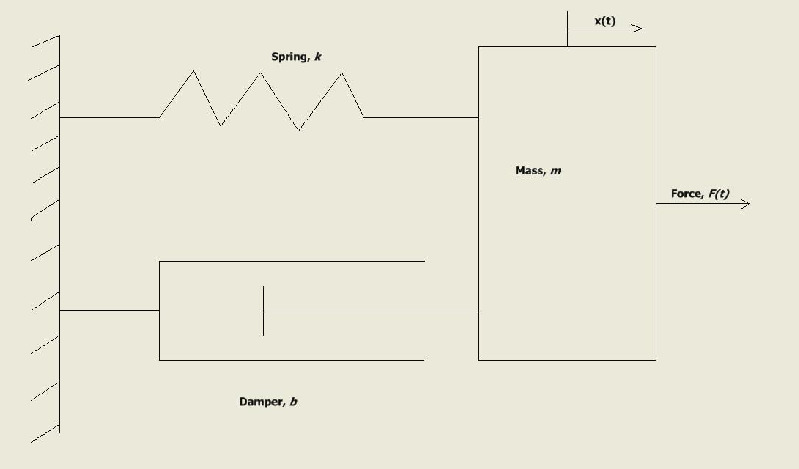
\includegraphics[height=5em,width=10em]{figures/spring-mass-damper.jpg} & 
		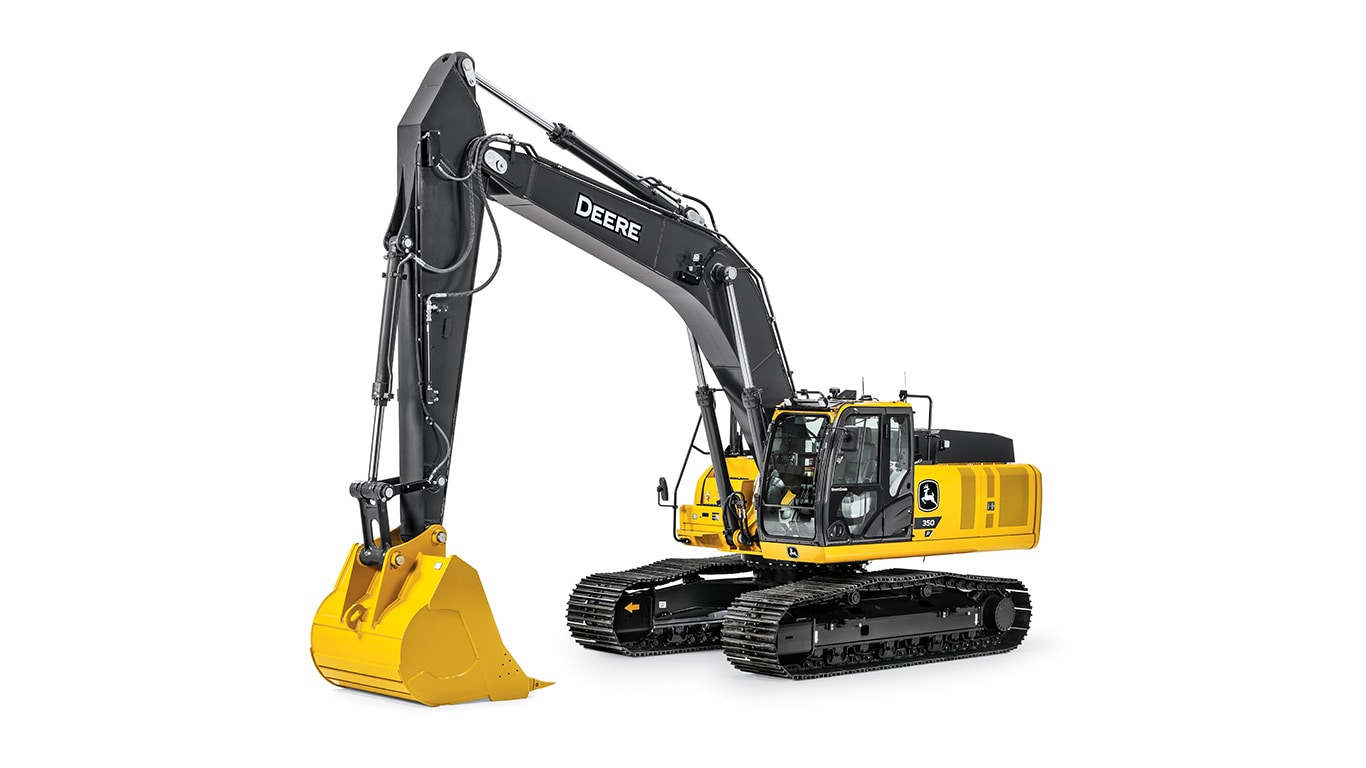
\includegraphics[height=5em,width=10em]{figures/excavJohnDeere.jpg} \\
		\hline \\
		Car suspension & Daimler  Plant \\
		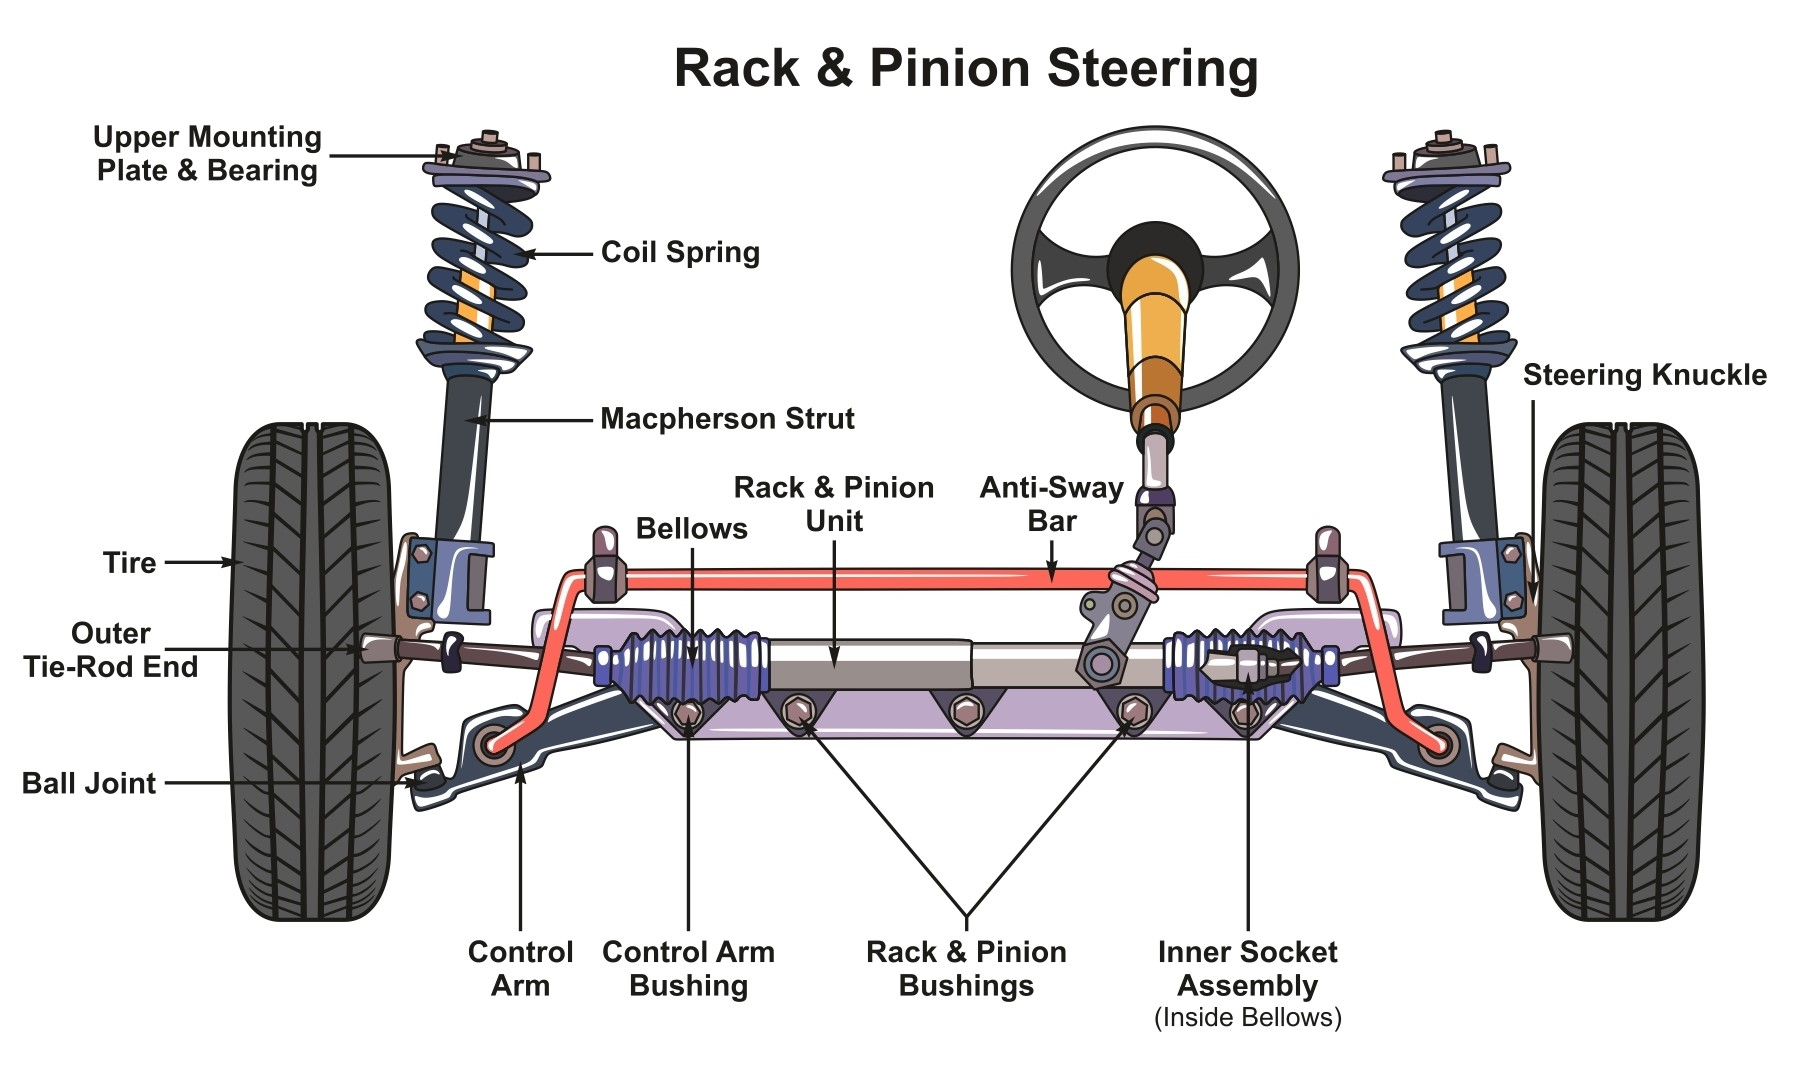
\includegraphics[height=5em,width=10em]{figures/carsusp.jpg} &
		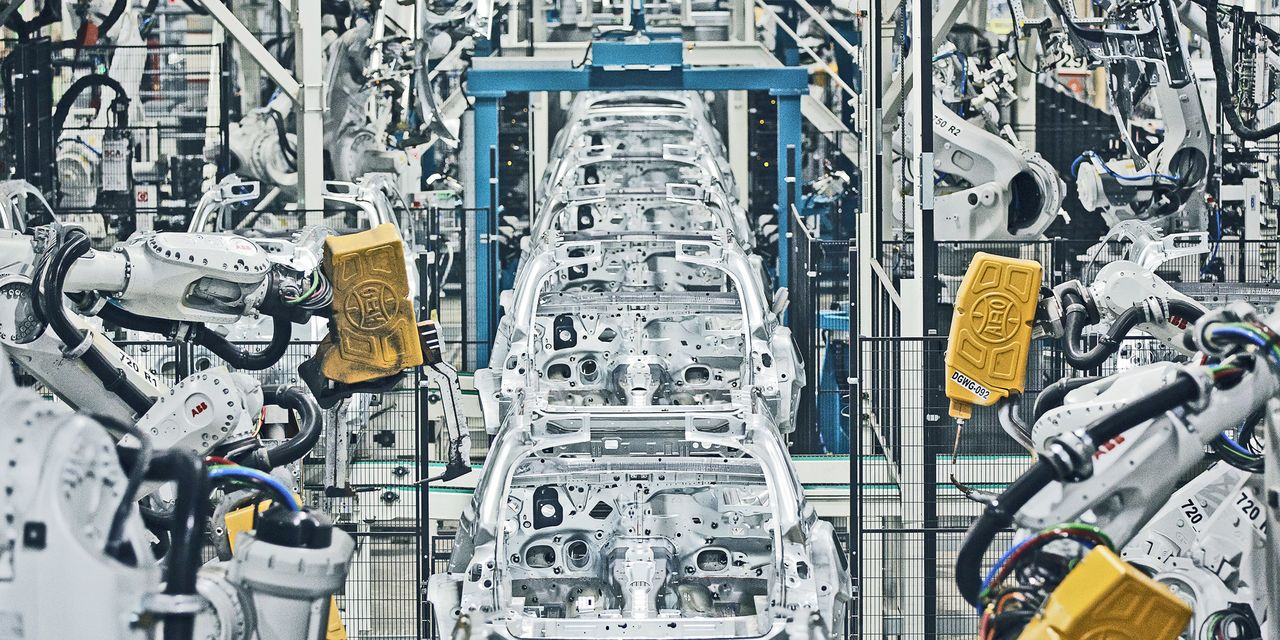
\includegraphics[height=5em,width=10em]{figures/daimler_manuf.jpeg} \\
		\hline
	\end{tabular}
\end{frame}

\subsection{Pairs and Linkages}
\begin{frame}
	\frametitle{Lower Pairs, Higher Pairs, Linkages}
	%
	\begin{block}{Lower and Higher Pairs}
		When elements of pairs touch one another over a \textcolor{red}{substantial region of a surface covering a line, curve-surface, or point of contact}, we have \textcolor{blue}{lower pairs}. When they touch \textcolor{red}{along a discrete line, curve-surface, or point of contact}, we have \textcolor{blue}{higher pairs}.
	\end{block}
	%
	\begin{block}{Linkage (Hunt, 1978)}
		If all joints of a \textcolor{red}{mechanism or mechanical movement} belong to lower pairs, we have a \textcolor{blue}{linkage}. 
	\end{block}
	%
\end{frame}

\begin{frame}
	\frametitle{Prismatic Pairs or $P$-pairs}
	%
	\begin{block}{Hunt, 1978}
		\footnotesize{Formed by receding the axis of the revolution surface between two pairs to $\infty$ so that the \textcolor{blue}{curve} that produces the surface moves parallel to itself, \textcolor{green}{tracing a cylinder}; or a \textcolor{blue}{polygonal-tracing curve} generates a \textcolor{green}{prism}.}
	\end{block}
	%
	\begin{columns}[t]		
		\begin{column}{.7\textwidth}
			\begin{figure}
				\centering
				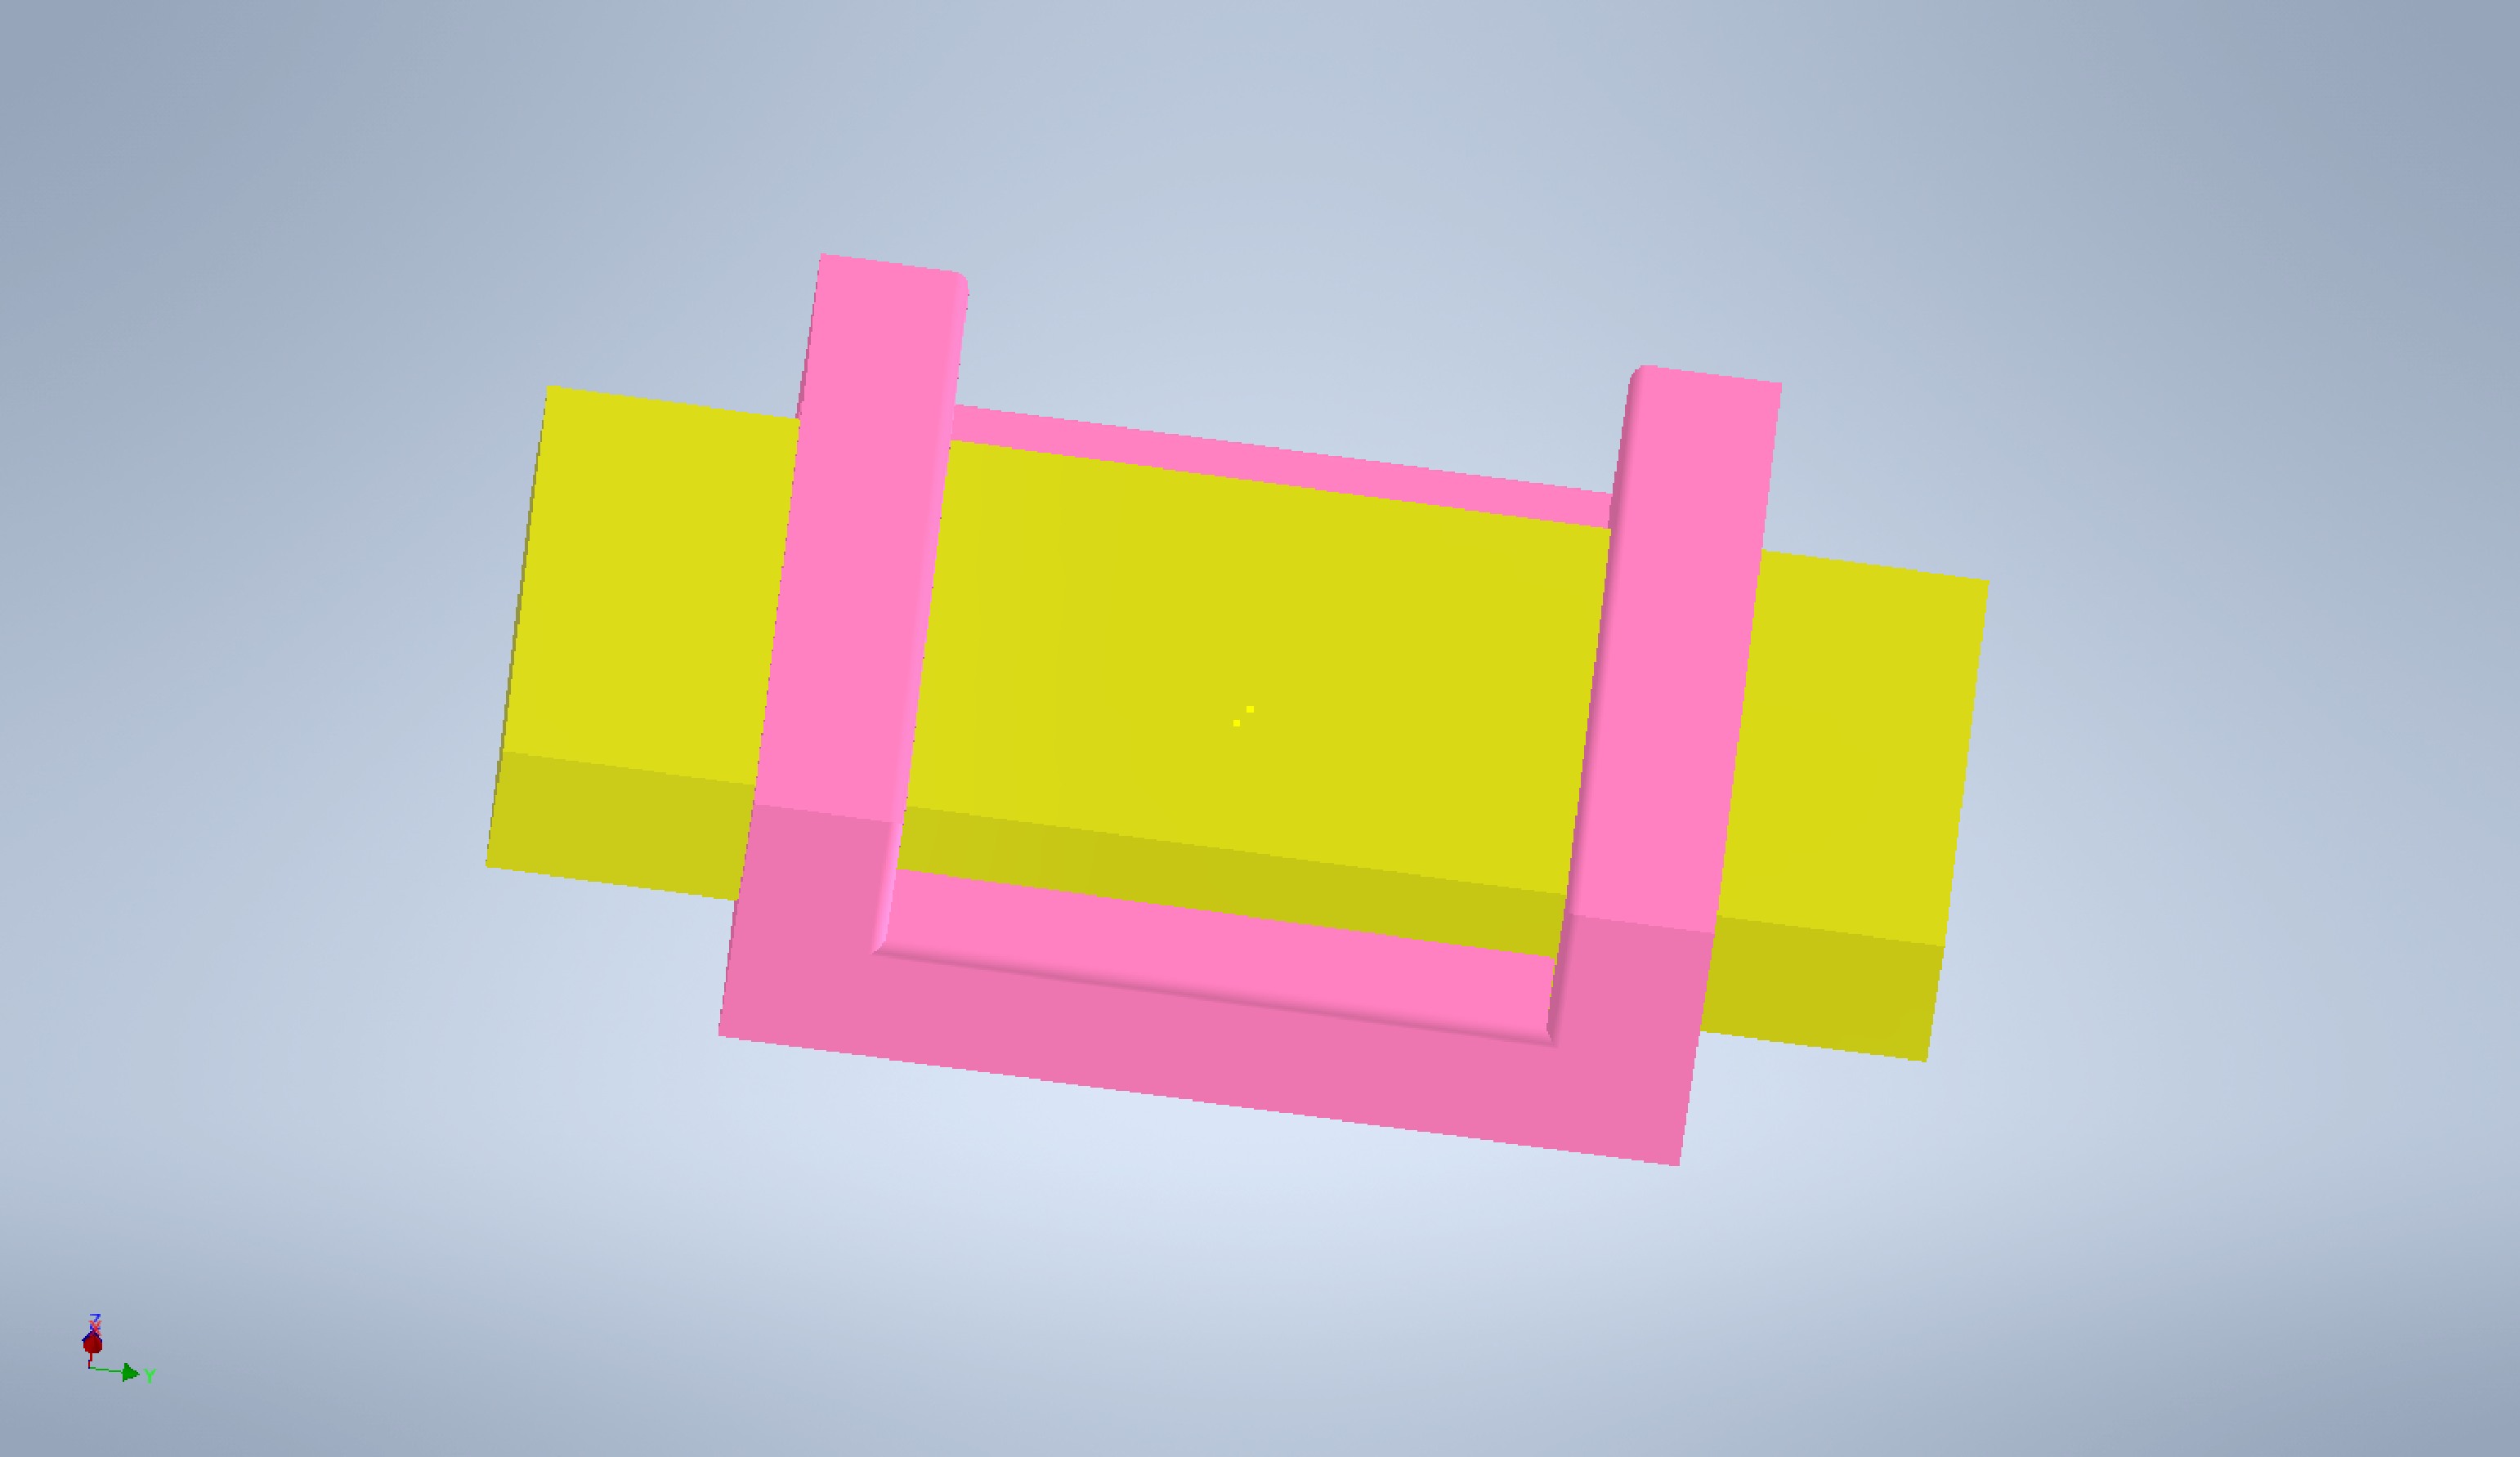
\includegraphics[width=\textwidth]{../Notes/figures/prismatic_joint.pdf}
			\end{figure}
		\end{column}
	\end{columns}
	%
	%\footnotesize{\textcolor{red}{Revolute} or \textcolor{red}{Hinge} or \textcolor{red}{Turning} or simply \textcolor{red}{$R$-pairs} with and without shoulder cutaway geometries. Credit: Wikimedia commons.}
\end{frame}

\begin{frame}
	\frametitle{Revolute Pairs or $R$-pairs}
	%
	\footnotesize{One \textcolor{red}{convex surface} and \textcolor{red}{one non-convex} surface for a \textcolor{green}{one degree of rotational freedom} around the one \textcolor{blue}{joint} the two surfaces make.}
	%\note{An R-pair has a convex and non-convex surface. Revolution surface can be traced by any general curve, outside a planar curve or a circle with axis of revolution about center as it produces an $S$-pair element.}
	\begin{columns}[t]		
		\begin{column}{.5\textwidth}
			\begin{figure}
				\centering
				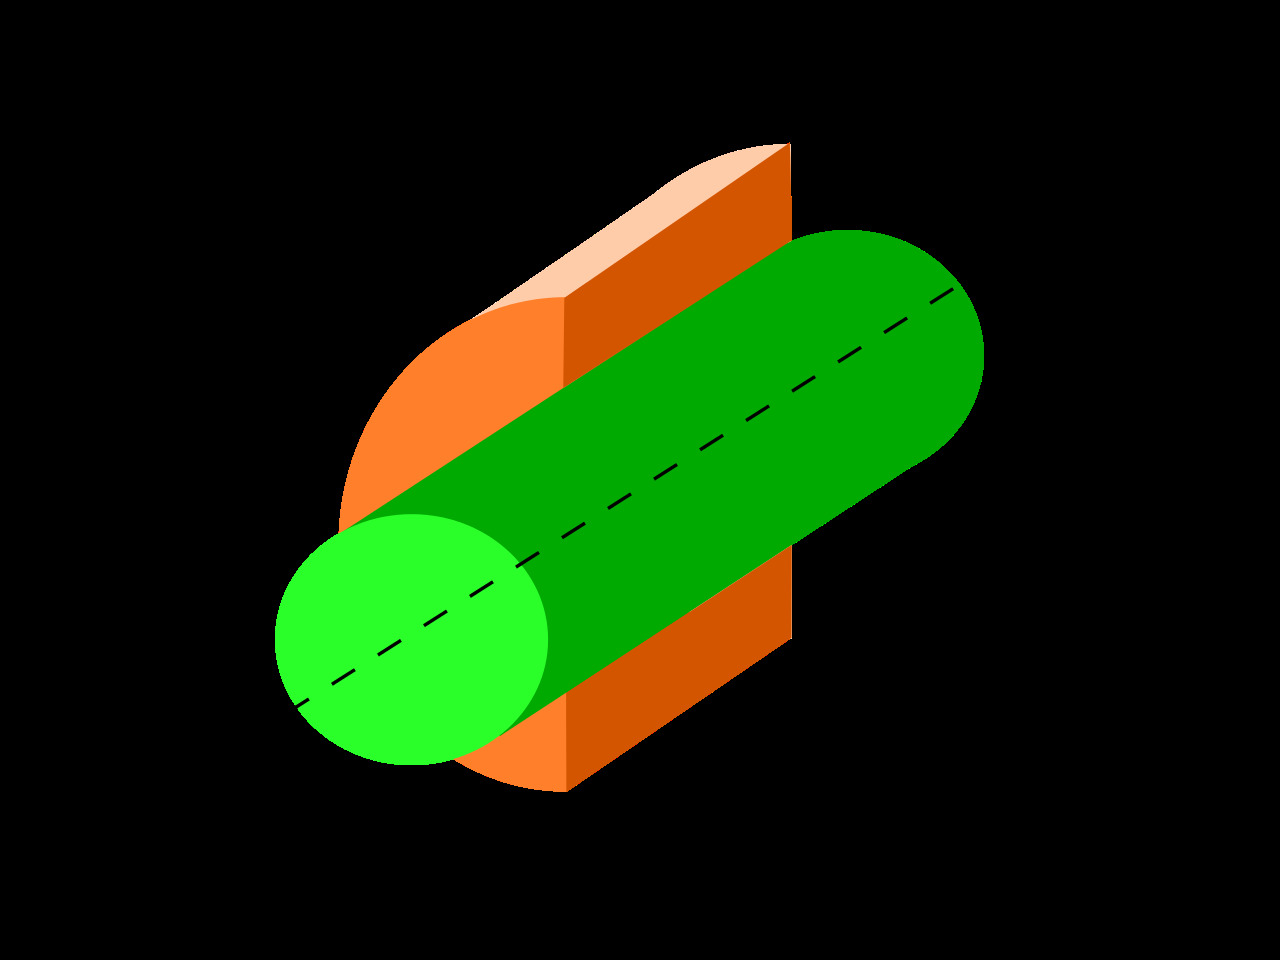
\includegraphics[width=\textwidth]{figures/revolute.jpg}
			\end{figure}
		\end{column}
		\begin{column}{.5\textwidth}
			\begin{figure}
				\centering
				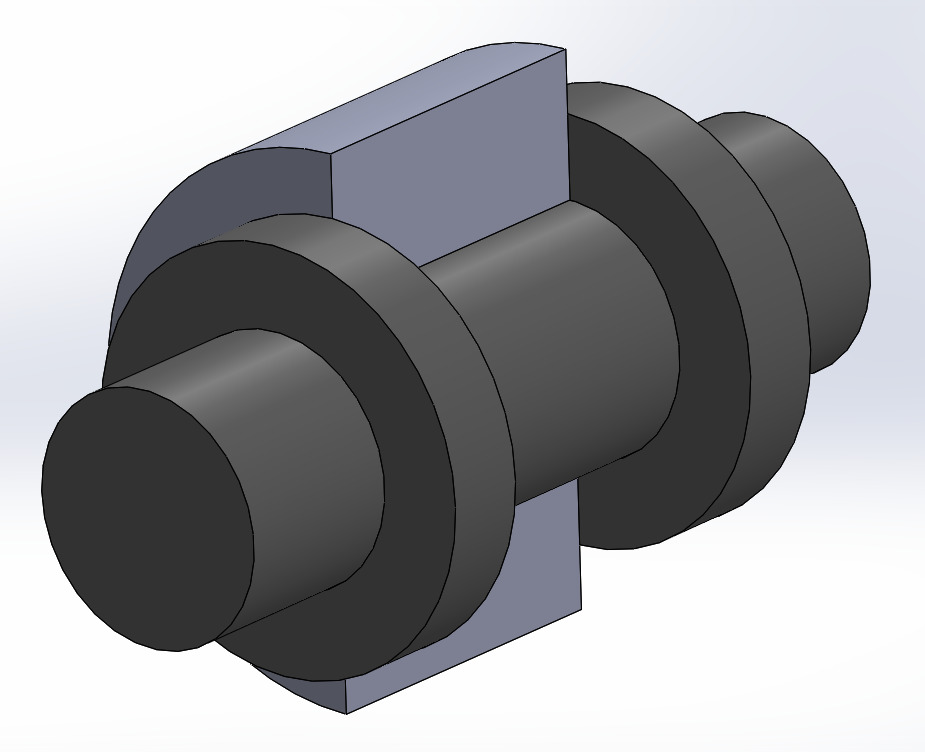
\includegraphics[width=\textwidth]{figures/revolute_cutaway.jpg}
			\end{figure}
		\end{column}
	\end{columns}
	%
	 \footnotesize{\textcolor{red}{Revolute} or \textcolor{red}{Hinge} or \textcolor{red}{Turning} or simply \textcolor{red}{$R$-pairs} with and without shoulder cutaway geometries. Credit: Wikimedia commons.}
\end{frame}


\begin{frame}
	\frametitle{Helical- \& U-Joints}
	%
	\begin{columns}[t]		
		\begin{column}{.5\textwidth}
			\begin{figure}
				\centering
				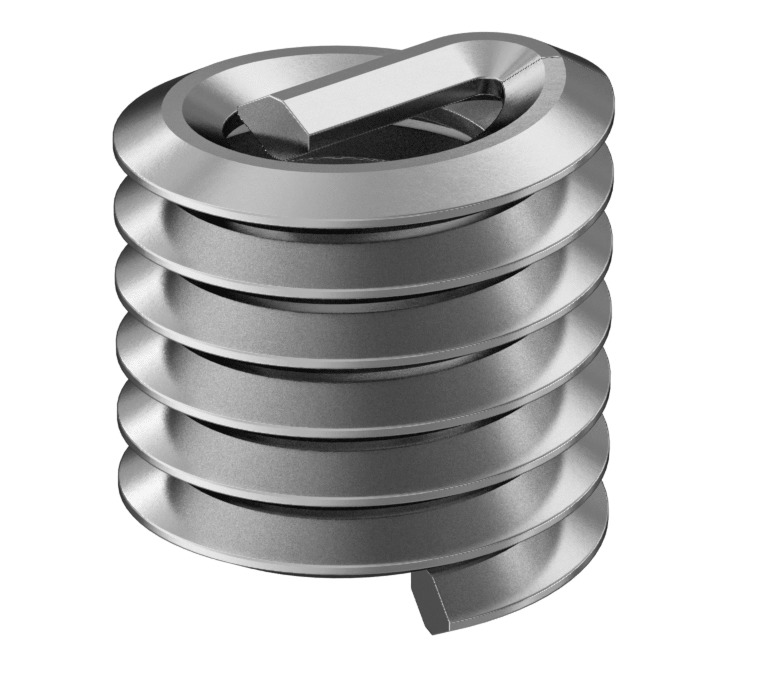
\includegraphics[width=\textwidth]{figures/helical.jpg}
			\end{figure}
			\centering Helical Joint
		\end{column}	
		\begin{column}{.5\textwidth}
			\begin{figure}
			\centering
			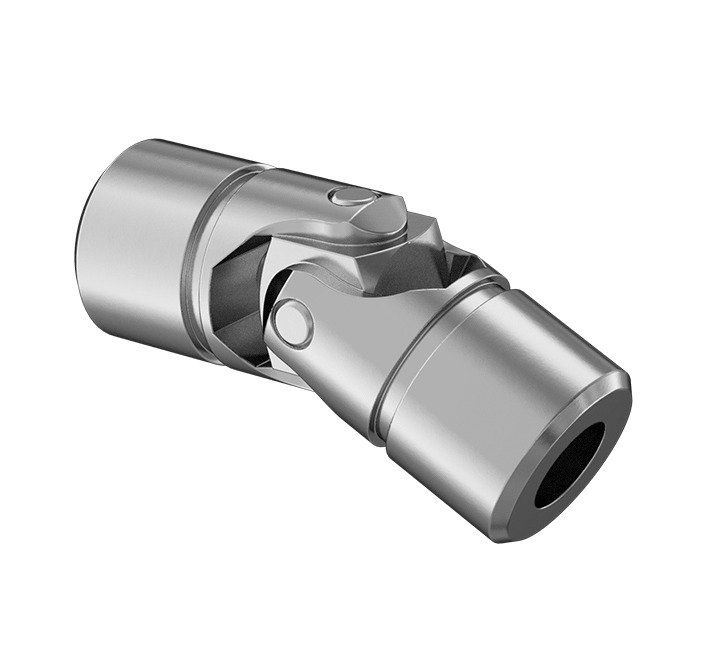
\includegraphics[width=\textwidth]{figures/ujoint.jpg}
			\end{figure}
			\centering Universal Joint
		\end{column}
	\end{columns}
	%
	\footnotesize{\copyright McMaster Carr, May 2022.}
\end{frame}


%\note{Introduce the concept of lower and higher pairs. Then explain a linkage.}



\begin{frame}
	\frametitle{Common Lower Kinematic Pairs}
	%
	\begin{figure}[t]
		\centering
		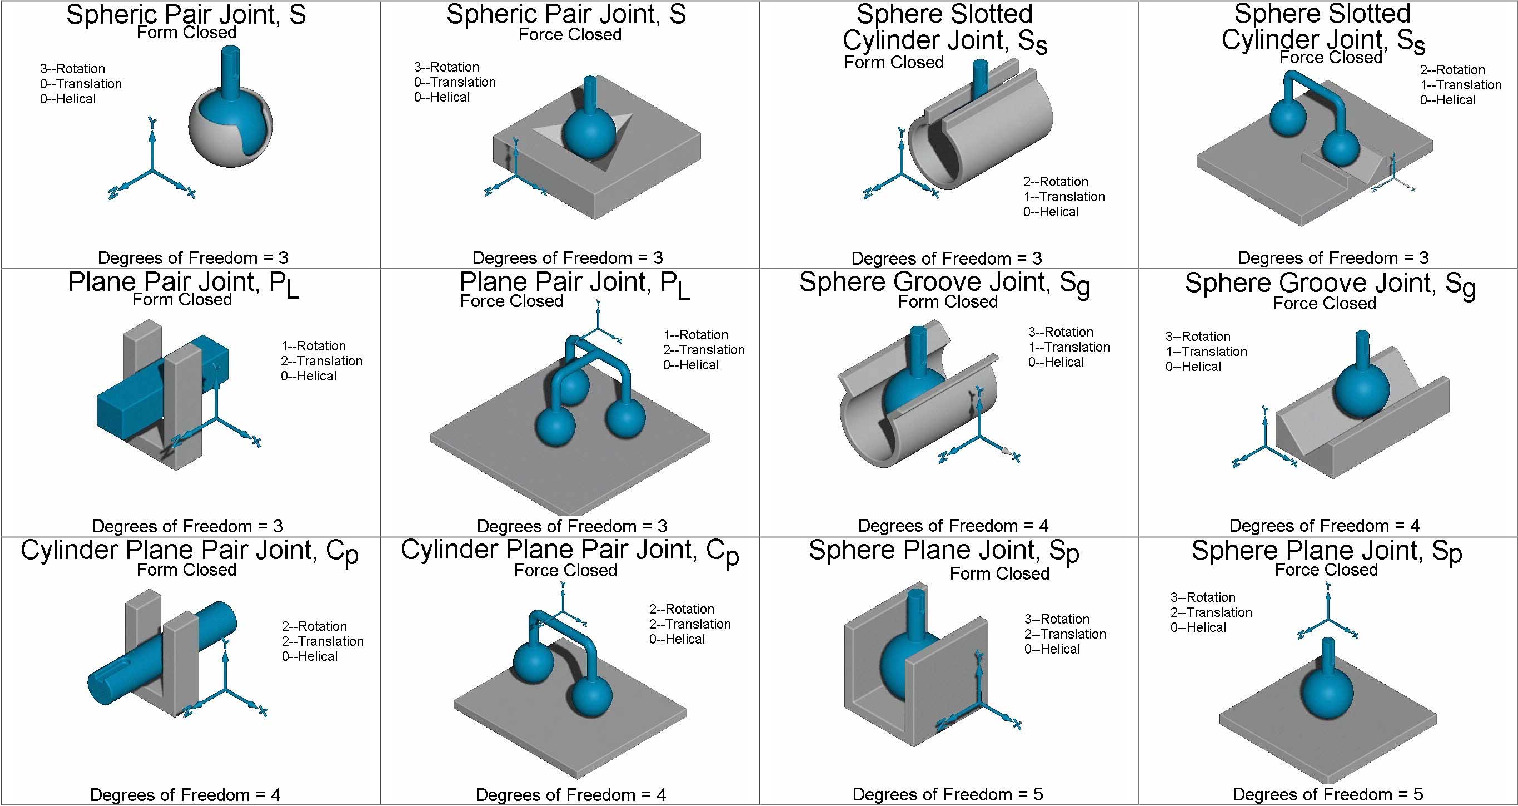
\includegraphics[width=\columnwidth]{figures/pairs2.jpg}
		Credit: \href{https://www.semanticscholar.org/paper/Development-of-Solid-Models-and-Multimedia-of-Pairs-Wharton-Singh/7ba9c2f3cfed5a493bb5828976689764d024b087}{\textcolor{blue}{Wharton and Singh,  2001}}.
	\end{figure}
\end{frame}


\begin{frame}
	\frametitle{Common Lower Kinematic Pairs}
	%
	\begin{figure}[t]
		\centering
		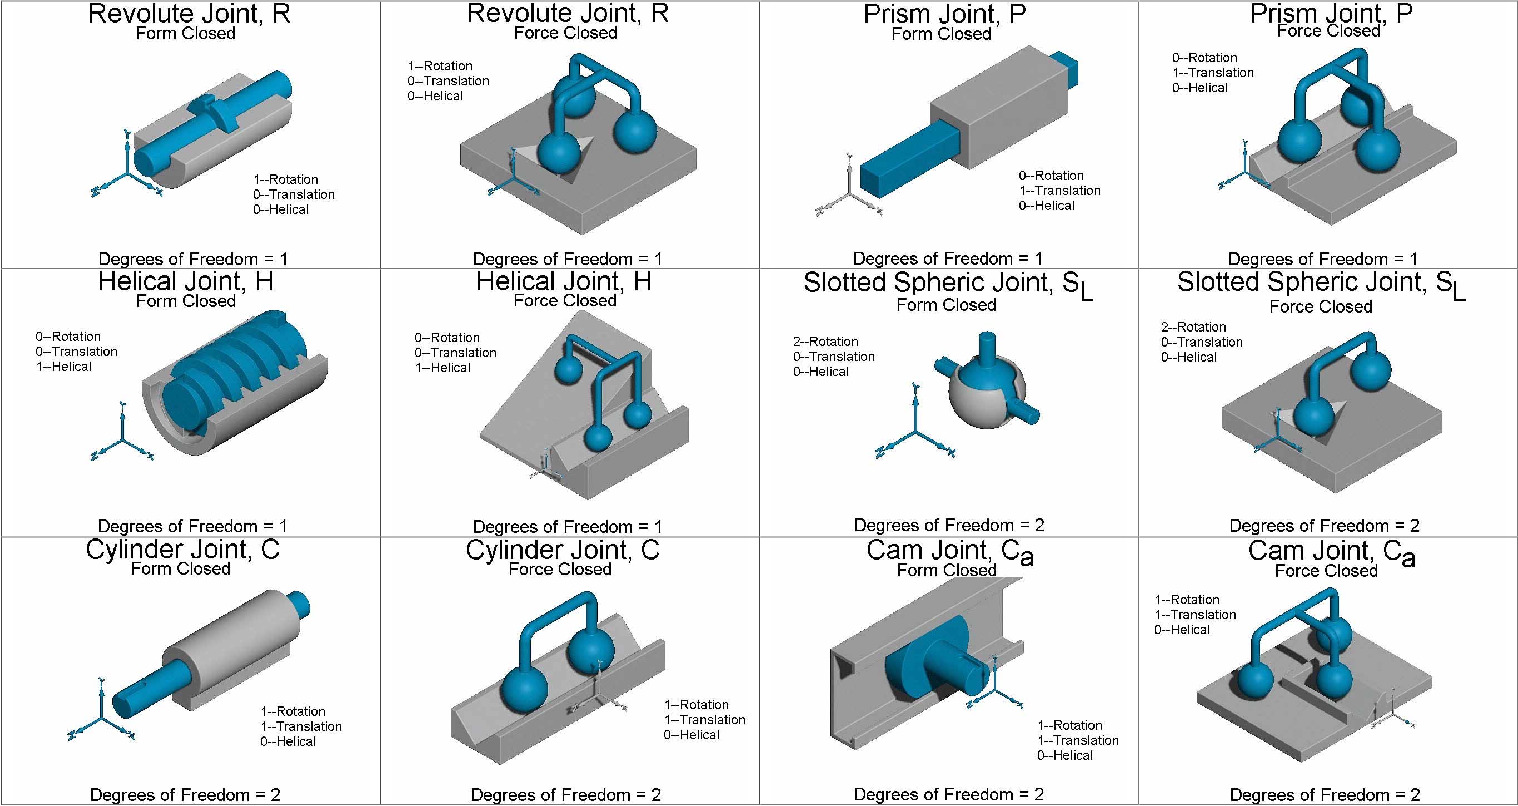
\includegraphics[width=\columnwidth]{figures/pairs.jpg}
		Credit: \href{https://www.semanticscholar.org/paper/Development-of-Solid-Models-and-Multimedia-of-Pairs-Wharton-Singh/7ba9c2f3cfed5a493bb5828976689764d024b087}{\textcolor{blue}{Wharton and Singh,  2001}}.
	\end{figure}
\end{frame}
	
	
\begin{frame}
	\frametitle{Kinematic Geometry of Common Actuations}
	\begin{block}{In-series vs. Parallel-actuated lower pairs}
		\begin{columns}[t]
			\begin{column}{10cm}
				\centering
				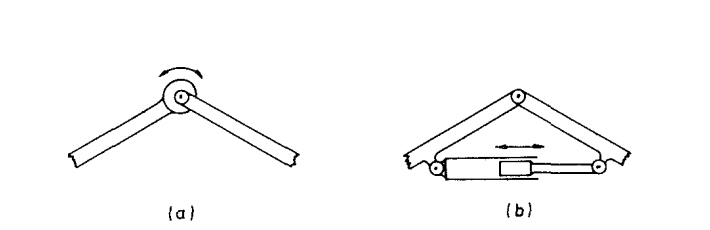
\includegraphics[width=\textwidth]{../Notes/figures/arms_hunt.png}
			\end{column}
		\end{columns}
		\footnotesize{(a): In-series-actuated kinematic pair with a rotary joint that is actuated ``about" the hinge. (b): Prismatic joint actuated ``across" a hinge. Reprinted from Hunt, Kenneth. Structural Kinematics of In-Parallel-Actuated Robot Arms. Transactions of ASME. 1983. }
	\end{block}
\end{frame}
		
\begin{frame}
	\frametitle{Kinematic Chains}
	%	
	\begin{block}{Kinematic Chains (Reuleaux, 1975)}
			We can explain the structural similarity of many mechanisms by parts of \textcolor{red}{kinematic chains} connected by pairs.
	\end{block}
	\begin{block}{Kinematic chains}
		\textcolor{blue}{Kinematic chains} are essentially the basic building structure of \textcolor{red}{mechanisms} $\ldots$ \textcolor{red}{and robots!} 
	\end{block}
\end{frame}
	
%\begin{frame}
%		\frametitle{Kinematic Chains}
%		%\begin{block}{.5\textwidth}
%		\begin{columns}[t]
%			\begin{column}{5cm}
%					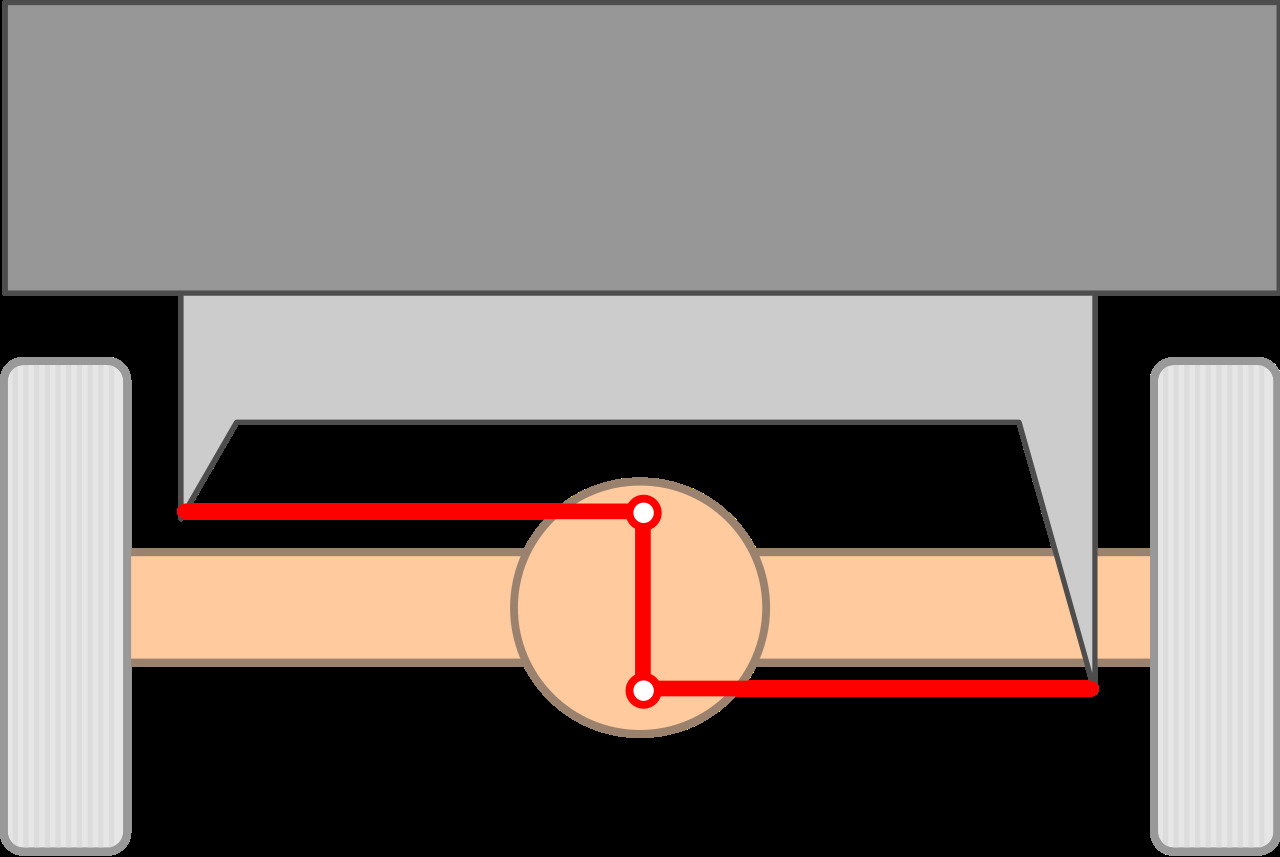
\includegraphics[width=1.5\textwidth, height=1.5\textwidth]{figures/WattsLinkage.jpg} 
%					\footnotesize{The Watt's Linkage Vehicle Suspension.} 
%		\end{column}
%			%	
%		\begin{column}{5cm}
%			\begin{minipage}[b]{.5\textwidth}
%				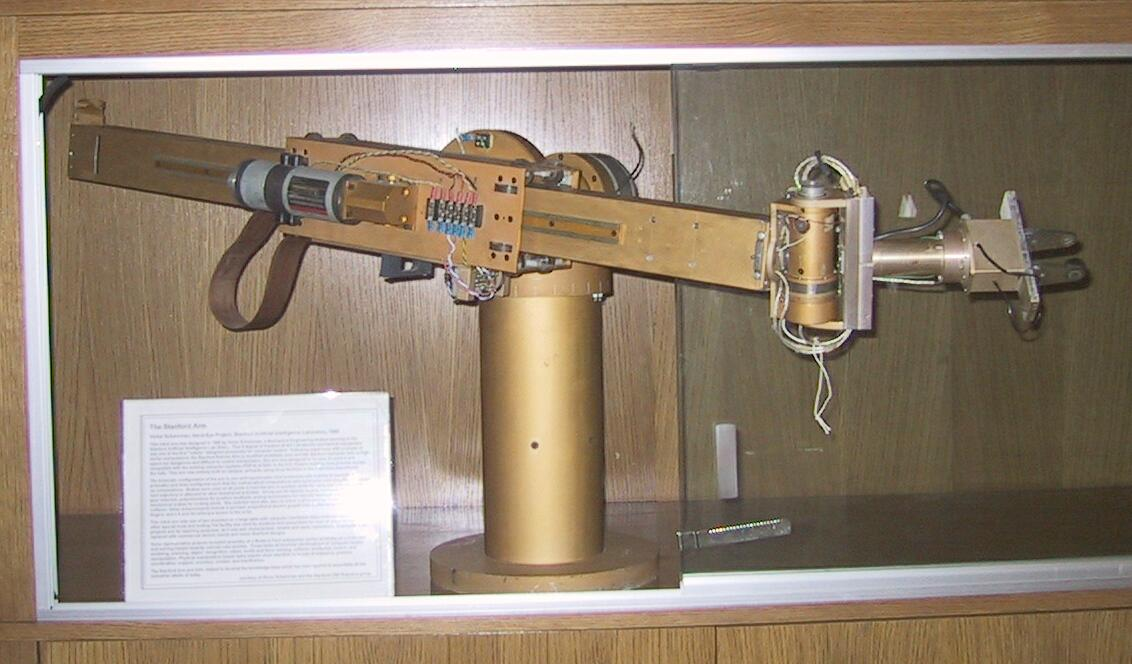
\includegraphics[width=1.5\textwidth, height=1.5\textwidth]{../Notes/figures/StanfordArm.jpg}  \\
%				\footnotesize The Stanford Arm (Infolab 1969). %Six degrees of freedom open kinematic chain.
%			\end{minipage}
%		\end{column}
%	\end{columns}
%%\end{block}
%\end{frame}

\subsection{Serial Chains}
	\begin{frame}
		\frametitle{Open Kinematic Chains}
		%	
		\begin{block}{Chains}
			Open kinematic chains are based off the anthropomorphic construction of the human hand with cantilevered beam structures.
		\end{block}
		\begin{block}{Chain Mechanisms and Error Amplification}
			Amplifies errors from waist (or base frame) all the way to the tool frame. Control difficult. 
		\end{block}
		%
		\begin{block}{Control}
			Feedforward control: High power and precision hydraulic actuators for servo motors. \\
			Sensory feedback control: Force sensing (Ernst, 1962). 
		\end{block}
	\end{frame}
	
	
	\note{The PUMA arm is the world's first serial kinematic chain. Developer: Victor Scheinman, Stanford student in the `50's. Made several iterations. Patent Rights: Joe Engelberger, (Danbury Unimation, 1961). Joe -- father of robotics -- created world's first robotics company in '61.}
	\begin{frame}
		\frametitle{Open Kinematic Robot Mechanisms}
		\begin{definition}[Ken Salisbury Jr., 1982]
			``\footnotesize \textit{[Robots are] our fascination with constructing mechanical analogues of ourselves... [this fascination] has led us to place all sorts of hopes and expectations in robot capabilities}."
		\end{definition}
		\begin{columns}[t]
			\begin{column}{5cm}
				\begin{minipage}[b]{.5\textwidth}
					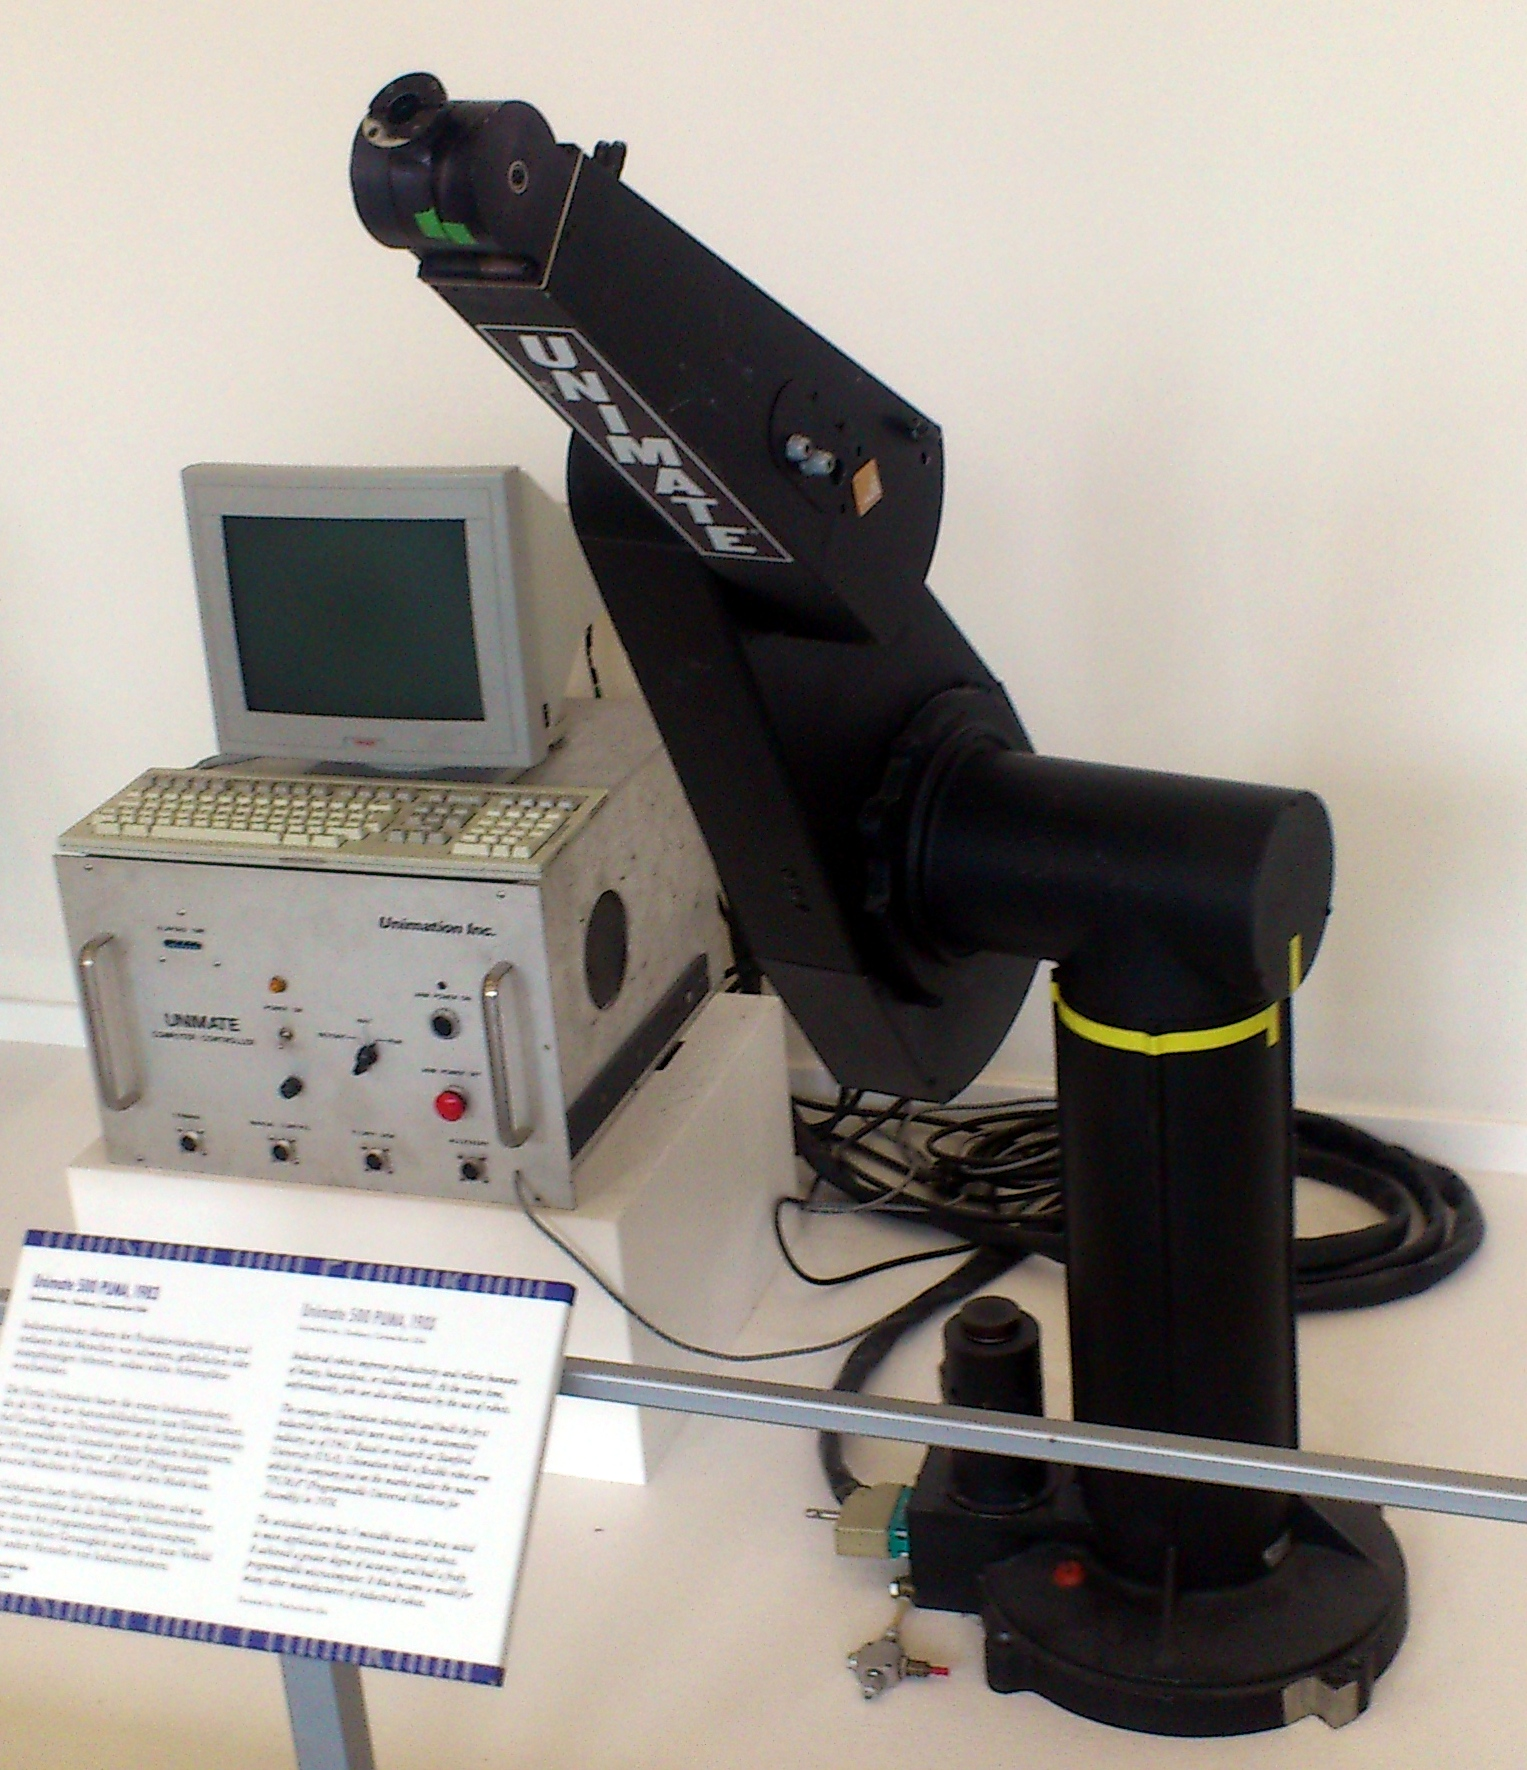
\includegraphics[width=1.5\textwidth, height=1.5\textwidth]{../Notes/figures/PUMA.jpg} \\
					\footnotesize{The St{\"a}ubli PUMA Robot (1956).} %Programmable Universal Manipulation Arm.}
			\end{minipage}
			%
		\end{column}	
		\begin{column}{5cm}
			\begin{minipage}[b]{.5\textwidth}
				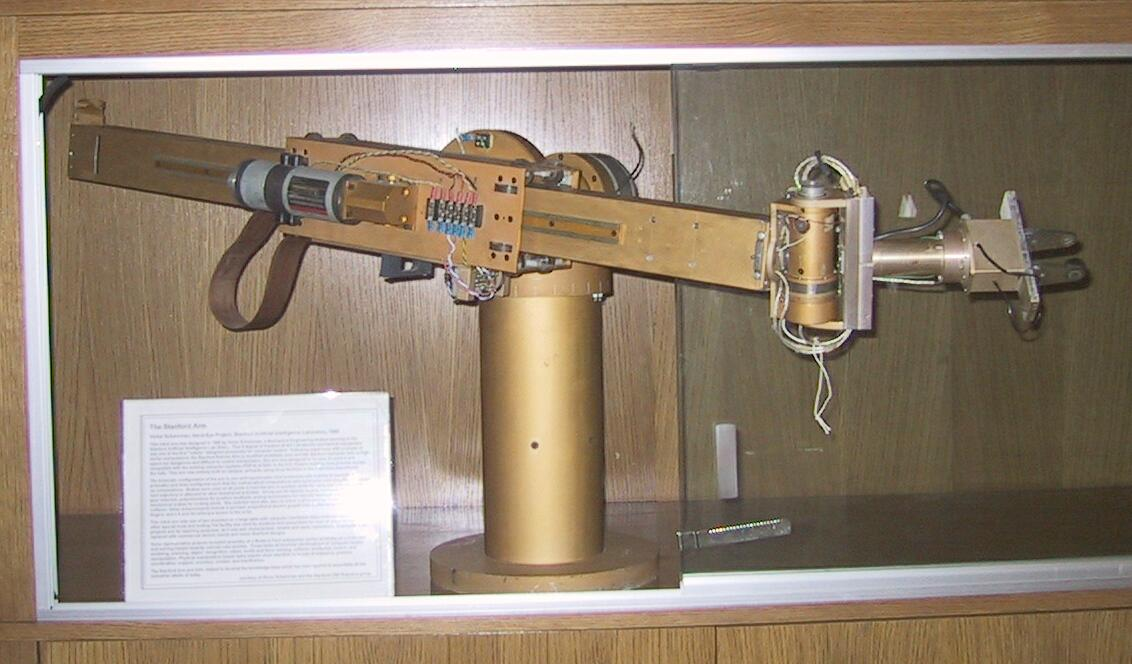
\includegraphics[width=1.5\textwidth, height=1.5\textwidth]{../Notes/figures/StanfordArm.jpg}  \\
				\footnotesize The Stanford Arm (Infolab 1969). %Six degrees of freedom open kinematic chain.
			\end{minipage}
		\end{column}
	\end{columns}
\end{frame}


\begin{frame}
\frametitle{Open Kinematic Chains}
%
\begin{tcolorbox}[coltitle=blue!80!yellow,colframe=brown!80]
	Open kinematic chains provide unstructured environmental interaction.
\end{tcolorbox}
\begin{tcolorbox}[coltitle=blue!80!yellow,colframe=gray!100]
	Project MAC, MIT.
\end{tcolorbox}
\begin{tcolorbox}[coltitle=blue!80!yellow,colframe=black!80]
	Tomovic and Boni's pressure sensed grasp.
\end{tcolorbox}
\begin{tcolorbox}[coltitle=blue!80!yellow,colframe=pink!100]
	Binary robot vision system (McCarthy et al, 1963).
\end{tcolorbox}
\end{frame}

\begin{frame}
\frametitle{Open Kinematic Chains}
%
\begin{tcolorbox}[coltitle=cyan!80,colframe=green!100]
	Stanford Manipulator.
\end{tcolorbox}
\begin{tcolorbox}[coltitle=blue!80!yellow,colframe=blue!100]
	Boston arm.
\end{tcolorbox}
\begin{tcolorbox}[coltitle=blue!80!yellow,colframe=red!100]
	The AMF (American Machines and Foundry) arm.
\end{tcolorbox}
\begin{tcolorbox}[coltitle=blue!80!yellow,colframe=yellow!100]
	General electric's walking robot (1969).
\end{tcolorbox}
\end{frame}


\begin{frame}
\frametitle{Long Walk Towards Direct Drive Robot Arms}

\begin{tcolorbox}[coltitle=magenta!80!green,colframe=yellow!80!green]
	The 50's, 60's nd 70's witnessed use of hydraulics  for (feedforward) position control.
\end{tcolorbox}

\begin{tcolorbox}[coltitle=magenta!80!green,colframe=blue!80!green] 
	For feedback control, force sensors and pressure sensors were used in closed-loop scenarios.
\end{tcolorbox}

\begin{tcolorbox}[coltitle=magenta!80!green,colframe=red!80!green] 
	Electrical actuation meant that robots had to be operated at high speeds. Needs for gear reduction for safe operations at low speeds. 
\end{tcolorbox}

\begin{tcolorbox}[coltitle=magenta!80!green,colframe=brown!80!green]
	With gear reduction came backlash, friction, and associated expenses.
\end{tcolorbox}
\end{frame}


\note{CMU DD I/II Arms: Workspace is donut shaped. OD:  90cm; ID: 21.7cm; $1.8m^2$ workspace area. Built by Harry Asada. Structural design similar to aircraft gimbal arm; Uses Samarium Cobalt rare earth magnet brushless DC motors on first 3 joints, and AlNiCo magnets on tip joints. No belts, transmissions making for faster transmitting of motions, less friction, low energy, low compliance. Each joint has complex AL housing which enables: (i) Control of geometrical relationships of bearing assembly; (ii) Control of servo components to bearing assembly; (iii) Controls of rotational axes to consecutive joints.}


\begin{frame}
\frametitle{Direct Drive Robot Mechanism: CMU DD I Arm}
\begin{tcolorbox}[coltitle=blue!80!yellow,colframe=brown!80!green]
	Along came Harry Asada.
\end{tcolorbox}
\begin{columns}[t]	
	%
	\begin{column}{.45\columnwidth}
		\begin{minipage}[b]{\textwidth}
			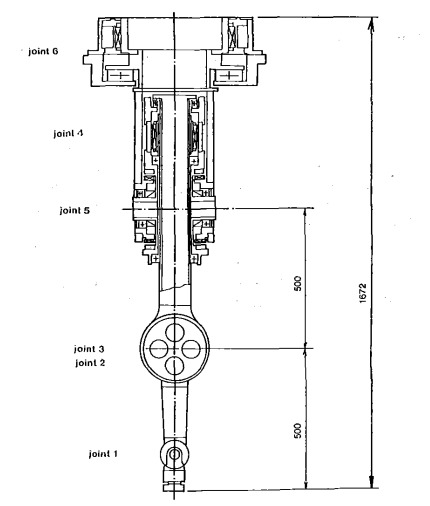
\includegraphics[width=1.2\textwidth, height=1.2\textwidth]{figures/cmu_arm.jpg} \\
			\footnotesize{Arm Schematics Transmission} %Programmable Universal Manipulation Arm.}
	\end{minipage}
	%
\end{column}
%
\begin{column}{.45\columnwidth}
	\begin{minipage}[b]{\textwidth}
		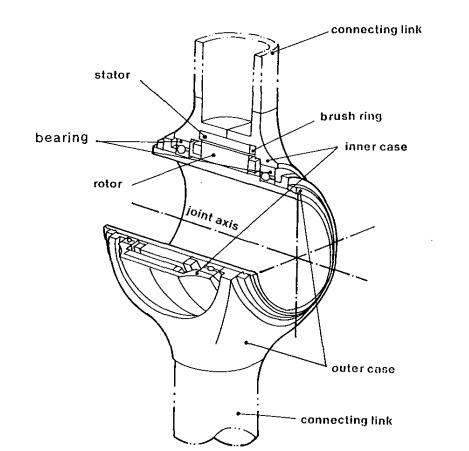
\includegraphics[width=1.2\textwidth, height=1.2\textwidth]{figures/dd_joints.jpg} \\
		\footnotesize{Joint schematic} %Programmable Universal Manipulation Arm.}
\end{minipage}
%
\end{column}
\end{columns}
\end{frame}

\begin{frame}
\frametitle{Direct Drive Robot Mechanism: CMU DD I Arm}
\begin{columns}[t]					%
%
\begin{column}{.45\columnwidth}
\begin{minipage}[b]{\textwidth}
	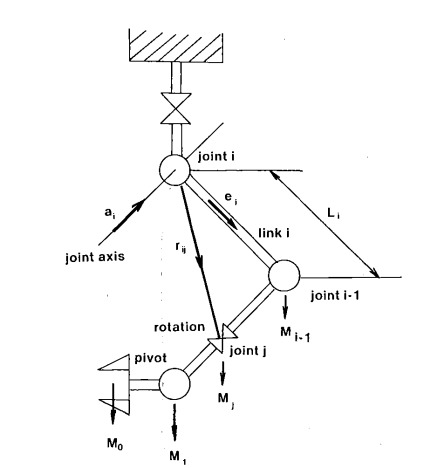
\includegraphics[width=1.1\textwidth, height=1.5\textwidth]{figures/dd_kinematics.jpg} \\
	\footnotesize{Kinematic model} %Programmable Universal Manipulation Arm.}
\end{minipage}
%
\end{column}
\begin{column}{.45\columnwidth}
\begin{minipage}[b]{\textwidth}
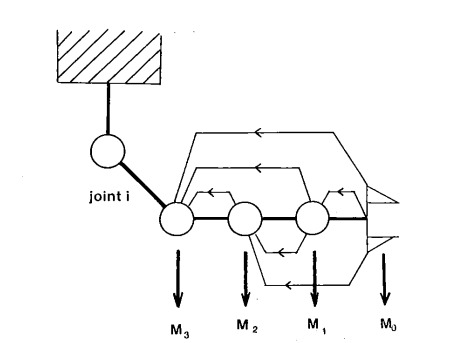
\includegraphics[width=1.2\textwidth, height=1.5\textwidth]{figures/dd_load_joints.jpg} \\
\footnotesize{Errors Transmission} %Programmable Universal Manipulation Arm.}
\end{minipage}
\end{column}
\end{columns}\end{frame}


\note{First direct-drive robot without a gearbox. Selective compliance in X-Y directions given its articulated jointed arms. One-freedom motion along $Z$ direction given its constrained arm New generations such as Cobra i600/i800 include power amplifiers, system and servo controls etc embedded in the robot's base. Kuka Scara arm: Lightweight, fast, powerful, low maintenance, energy consumption, investment costs etc.}
\begin{frame}
\frametitle{SCARA Robot Mechanisms}
\begin{columns}[t]	
\begin{column}{5cm}
\begin{minipage}[b]{.5\textwidth}
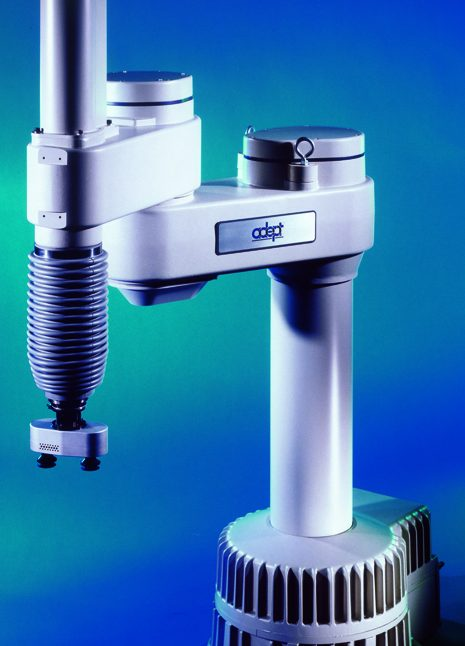
\includegraphics[width=1.5\textwidth, height=1.5\textwidth]{figures/adeptone.jpg}  \\
\footnotesize The Adept One SCARA robot (Debuted 1984). 
\end{minipage}
\end{column}
%
\begin{column}{5cm}
\begin{minipage}[b]{.5\textwidth}
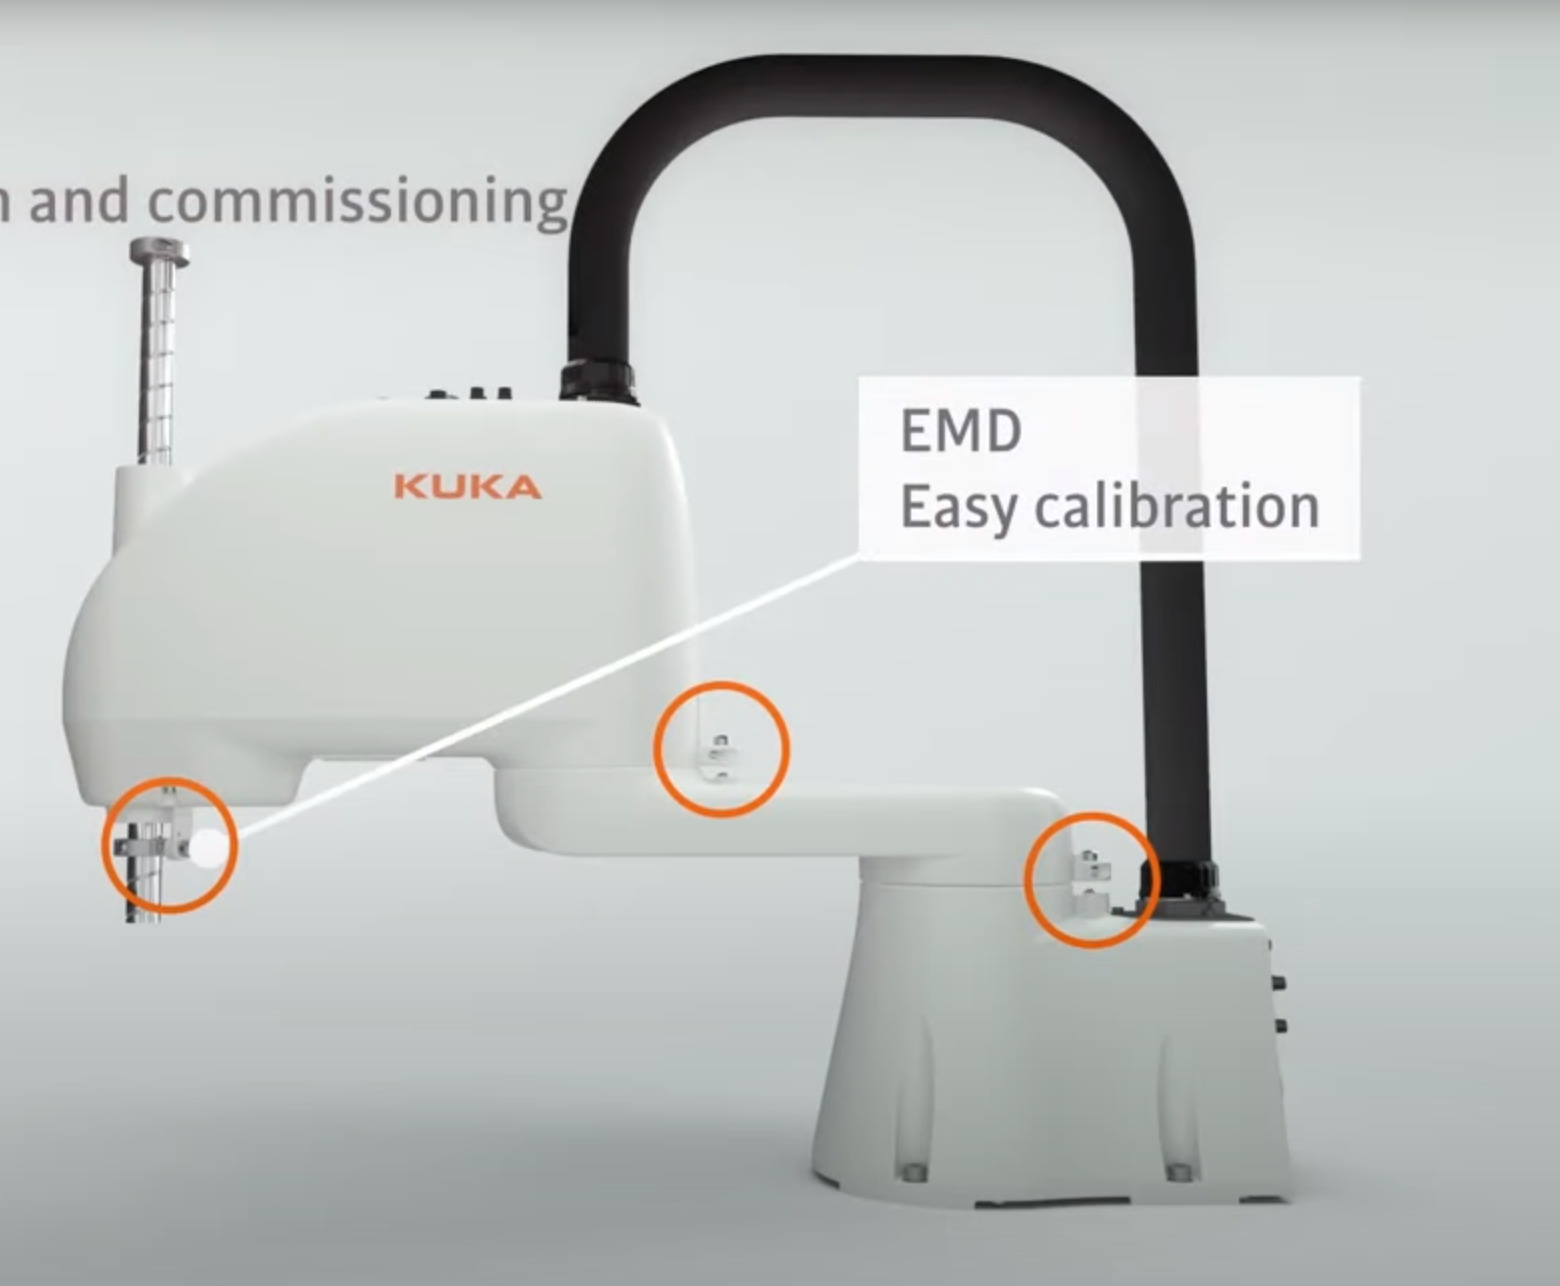
\includegraphics[width=1.5\textwidth, height=1.5\textwidth]{figures/Scara.jpg} \\
\footnotesize{Kuka's SCARA arm, 2022. \copyright Kuka Robotics} %Programmable Universal Manipulation Arm.}
\end{minipage}
%
\end{column}
\end{columns}
\end{frame}


\begin{frame}
	\begin{block}{The St{\"a}ubli anthropomorphic arm.}
		\begin{columns}[t]
			\begin{column}{10cm}
				\centering
				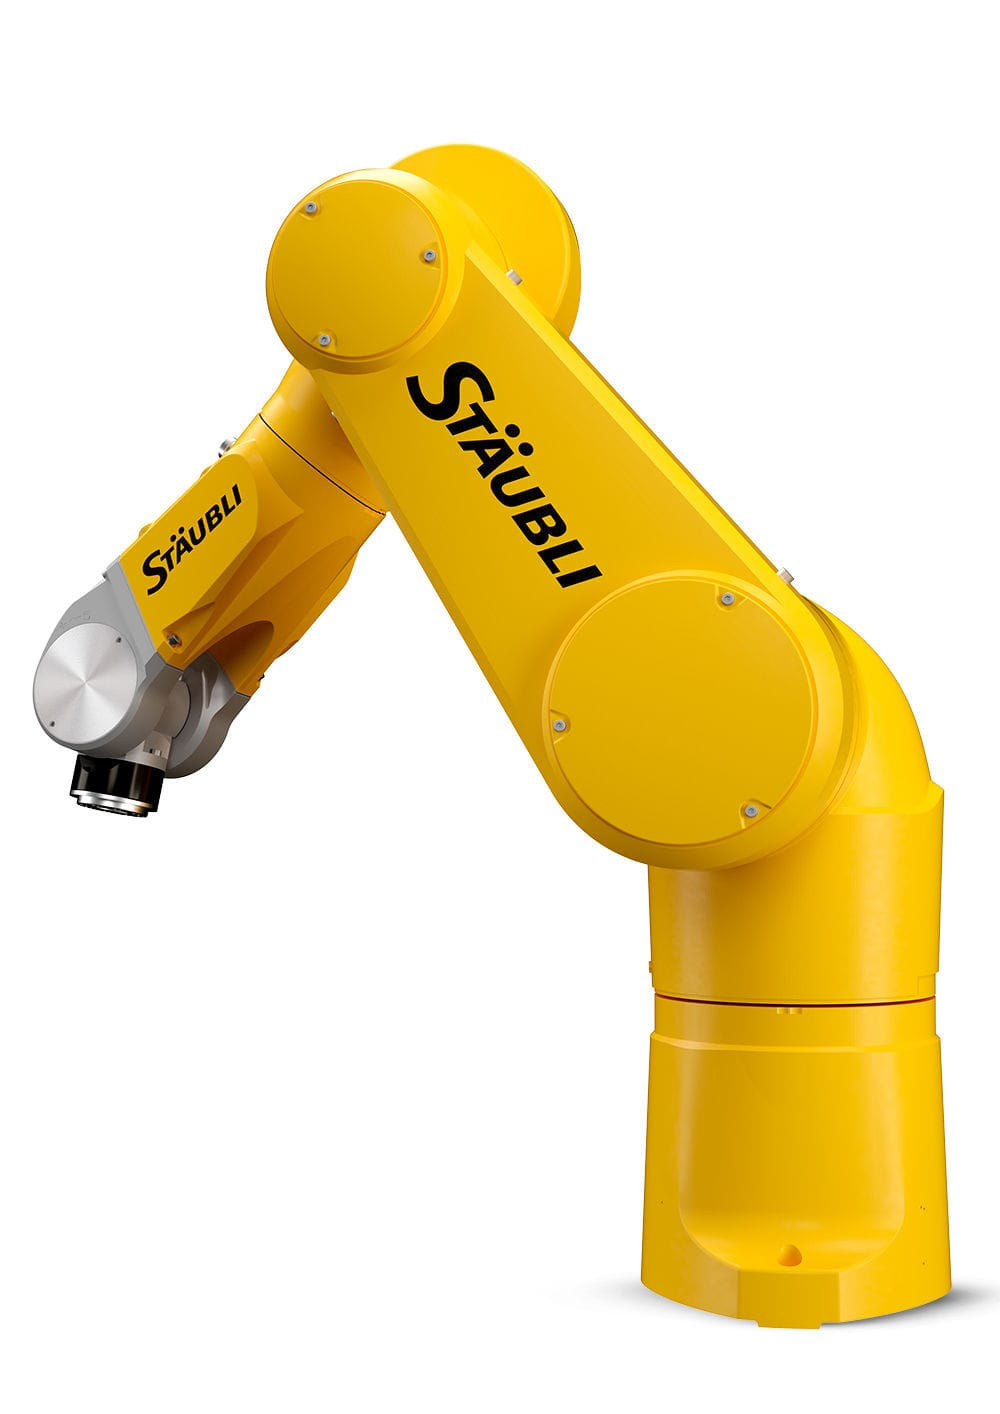
\includegraphics[scale=.1, width=.5\textwidth, rotate=-90]{../Notes/figures/Staubli.jpg}
			\end{column}
		\end{columns}
		\footnotesize{The Staubli 6-DOF Arm is an example of a Spherical Manipulator. Reprinted from DirectIndustry's Webpage.}
	\end{block}
\end{frame}

\begin{frame}
\frametitle{Serial mechanisms research in the 80's}
%
\tcbset{coltitle=cyan!80,colframe=gray!80!green,title=Mechanisms in the 80's,
enlarge left by=-5mm,enlarge right by=0mm,width=\linewidth+5mm}
\begin{tcolorbox}[toggle enlargement=none]
With the 80's came the arrival of PCs. Lots of research went into computational algorithms for the kinematics and kinetics of (mostly) anthropomorphic robot arms.
\end{tcolorbox}
\begin{tcolorbox}[coltitle=magenta!70,colframe=blue!80!red,title=Active control schemes,toggle enlargement=forced]
Efficient recursive Lagrangian and computational methods for the gravitational and Coriolis forces in Newton-Euler equations.
\end{tcolorbox}
\begin{tcolorbox}[coltitle=pink!70,colframe=gray!80!red,title=Feedback Linearization,toggle enlargement=evenpage]
Dynamics feedback linearization for precise bounds on manipulator performance.
\end{tcolorbox}
\end{frame}

\begin{frame}
\frametitle{Serial mechanisms research in the 90's}
%
\tcbset{coltitle=pink!80,colframe=gray!80,title=Robotworld,
enlarge left by=-5mm,enlarge right by=0mm,width=\linewidth+5mm}
\begin{tcolorbox}[title=Automatix,toggle enlargement=none]
Reconfigurable robots for various assembly ops.
\end{tcolorbox}
\begin{columns}[b]
\begin{column}{.48\columnwidth}			
\begin{tcolorbox}[colframe=blue!80!green, coltitle=white!80,toggle enlargement=none]
First industrial-scale re-configurable robot and with machine vision components. RAIL scripting OS originally based on Motorola 68000, later on replaced by Apple Macintosh II. 
\end{tcolorbox}
\end{column}
\begin{column}{.52\columnwidth}
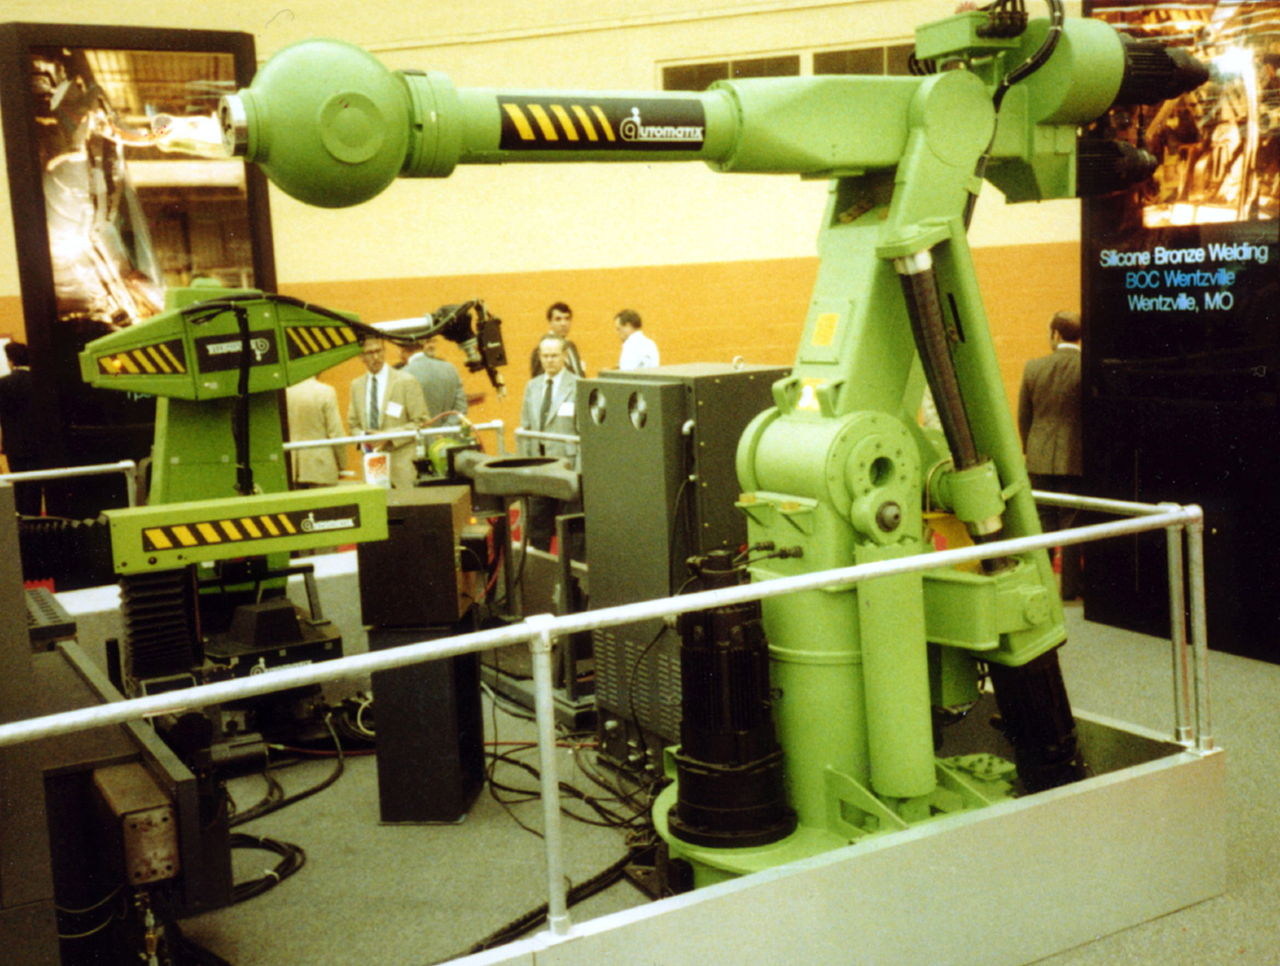
\includegraphics[width=\textwidth]{figures/Automatix.jpg}
\copyright Wikipedia
\end{column}
\end{columns}
\end{frame}

\subsection{Hyperredundant and Parallel robots}
	\begin{frame}
		\frametitle{Hyper-redundant Continuum Robots}
		\begin{columns}[b]
			\begin{column}{.33\columnwidth}			
				\begin{tcolorbox}[colframe=blue!80!green, coltitle=white!80,toggle enlargement=none]
					\centering 
					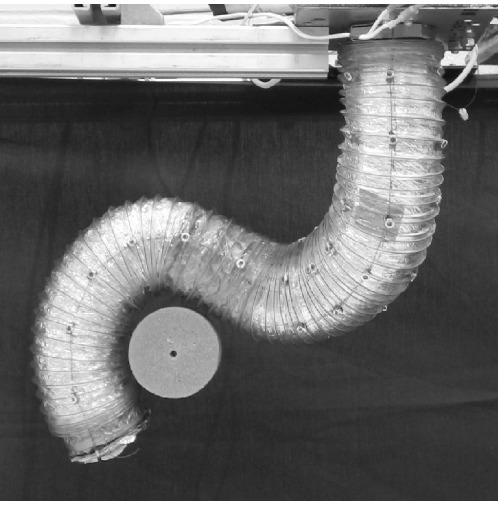
\includegraphics[width=\textwidth, height=1.1\textwidth]{figures/multisec_continuum.jpg}
				\end{tcolorbox}
			\end{column}	
		\begin{column}{.33\columnwidth}			
			\begin{tcolorbox}[colframe=blue!80!green, coltitle=white!80,toggle enlargement=none]
			\centering 
			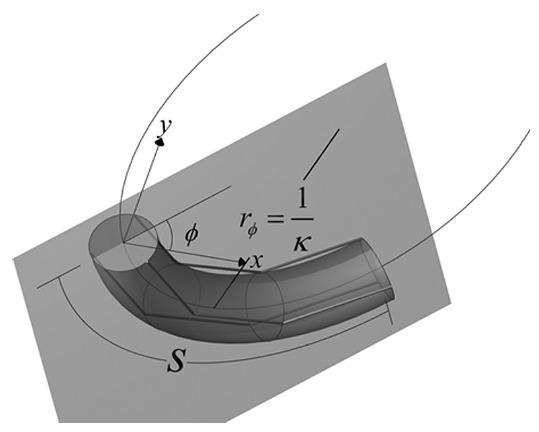
\includegraphics[width=\textwidth, height=1.1\textwidth]{figures/multi_sec_manip.jpg}
			\end{tcolorbox}
		\end{column}	
		\begin{column}{.33\columnwidth}			
			\begin{tcolorbox}[colframe=blue!80!green, coltitle=white!80,toggle enlargement=none]
			\centering 
			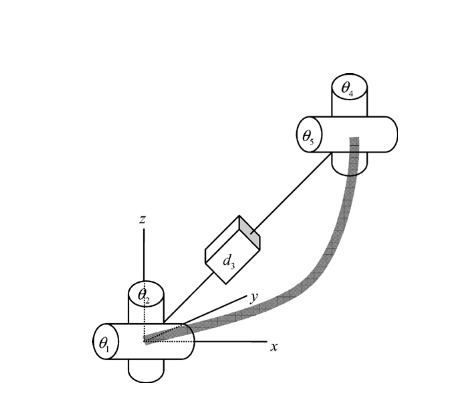
\includegraphics[width=\textwidth, height=1.1\textwidth]{figures/multi_sec_scheme.jpg}
			\end{tcolorbox}
		\end{column}	
		\end{columns}
		\centering \footnotesize{The elephant trunk continuum robot. Jones \& Walker, T-RO 2006. Inspiration: Muscular hydrostats in nature.}
	\end{frame}

\begin{frame}
	\frametitle{Hyper-redundant Kinematic Chains}
	\begin{columns}[b]
		\begin{column}{.98\columnwidth}			
			\begin{tcolorbox}[colframe=blue!80!green, coltitle=white!80,toggle enlargement=none]
				\centering 
				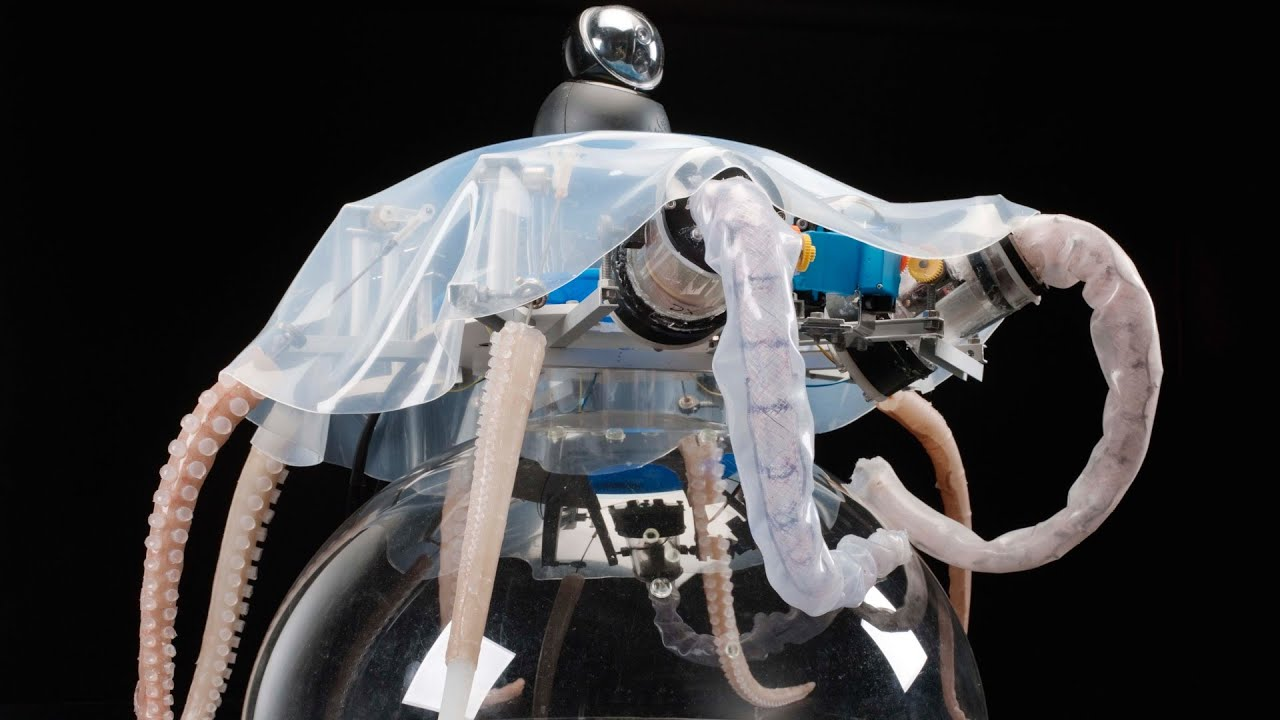
\includegraphics[width=\textwidth]{../Notes/figures/octopus.jpg}
			\end{tcolorbox}
		\end{column}	
	\end{columns}
	 \centering \footnotesize{An octopus-inspired soft robot. \copyright Cecilia Laschi.}
\end{frame}
	
	
	\begin{frame}
		\frametitle{Parallel Robots}
		%
		\tcbset{coltitle=pink!100,colframe=cyan!50,title=Robotworld,
			enlarge left by=-5mm,enlarge right by=0mm,width=\linewidth+5mm}
		\begin{tcolorbox}[title=Mehlet 2015,toggle enlargement=none]
			A \textcolor{blue}{parallel robot} is made up of an end-effector with n degrees of freedom, and of a fixed base, linked together by at least two independent kinematic chains. Actuation takes place through n simple actuators.
		\end{tcolorbox}	
	\end{frame}
	
	\begin{frame}
		\frametitle{Parallel mechanisms: Stewart-Gough Platforms}
		\footnotesize{Principles of a moving platform to test tyre wear and tear (Gough, 1947). Prototype, 1955.}
		\newline
		\begin{columns}[b]
			\begin{column}{.48\columnwidth}			
				\begin{tcolorbox}[colframe=blue!80!green, coltitle=white!80,toggle enlargement=none]
					\centering 
					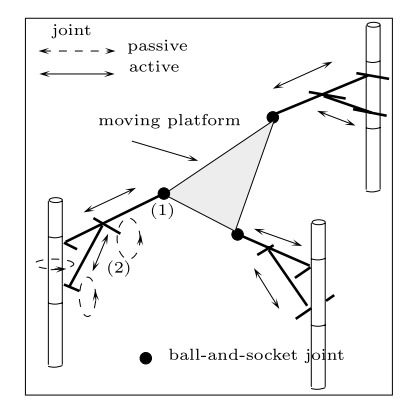
\includegraphics[width=\textwidth]{figures/Stewart.jpg}
				\end{tcolorbox}
			\end{column}
			\begin{column}{.48\columnwidth}			
				\begin{tcolorbox}[colframe=blue!80!green, 	coltitle=white!80,toggle enlargement=none]
				\centering 
				\includegraphics[width=.8\textwidth]{../../../Papers/PhDThesis/figures/GoughPlatform.jpg}
				\end{tcolorbox}
			\end{column}	
		\end{columns}
		\centering \footnotesize{\textit{Left}: Stewart's 1965 mechanism. \textit{Right:} The original 1954 octahedral hexapod proposed by  Gough. Courtesy: Parallemic.org.}
	\end{frame}

\begin{frame}
	\frametitle{Truss Robots}
	\begin{columns}[b]
		\begin{column}{.7\columnwidth}			
			\begin{tcolorbox}[colframe=blue!80!green, coltitle=white!80,toggle enlargement=none]
				\centering 
				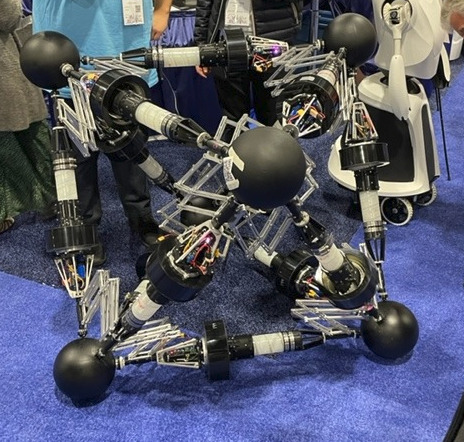
\includegraphics[width=.8\textwidth]{figures/truss.jpg}
			\end{tcolorbox}
		\end{column}	
	\end{columns}
	\centering \footnotesize{A multi-DOF Truss Robot. Courtesy of Penngineering (ICRA 2022, Philadelphia, PA).}
\end{frame}		
		
\begin{frame}
	\frametitle{Closed kinematic chains}
	\footnotesize{Connection degree $\ge 3$.}
	\newline
		\begin{columns}[b]
			\begin{column}{.74\columnwidth}			
				\begin{tcolorbox}[colframe=blue!80!green, coltitle=white!80,toggle enlargement=none]
					\centering 
					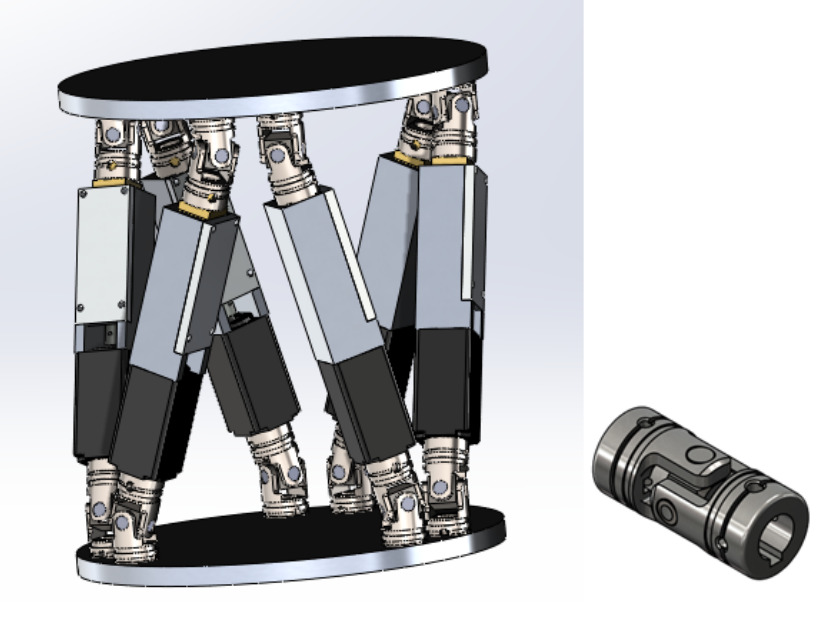
\includegraphics[width=\textwidth]{figures/stewart.jpg}
				\end{tcolorbox}
			\end{column}	
		\end{columns}
		\centering \footnotesize{A Stewart-Gough platform. SolidWorks Drawing Courtesy of Andrew Belcher. UChicago, 2018.}
\end{frame}

\begin{frame}
	\frametitle{A Soft Stewart Platform}
	\begin{columns}[b]
		\begin{column}{.8\columnwidth}		
			\begin{tcolorbox}[colframe=blue!80!green, coltitle=white!80,toggle enlargement=none]
				\centering 
				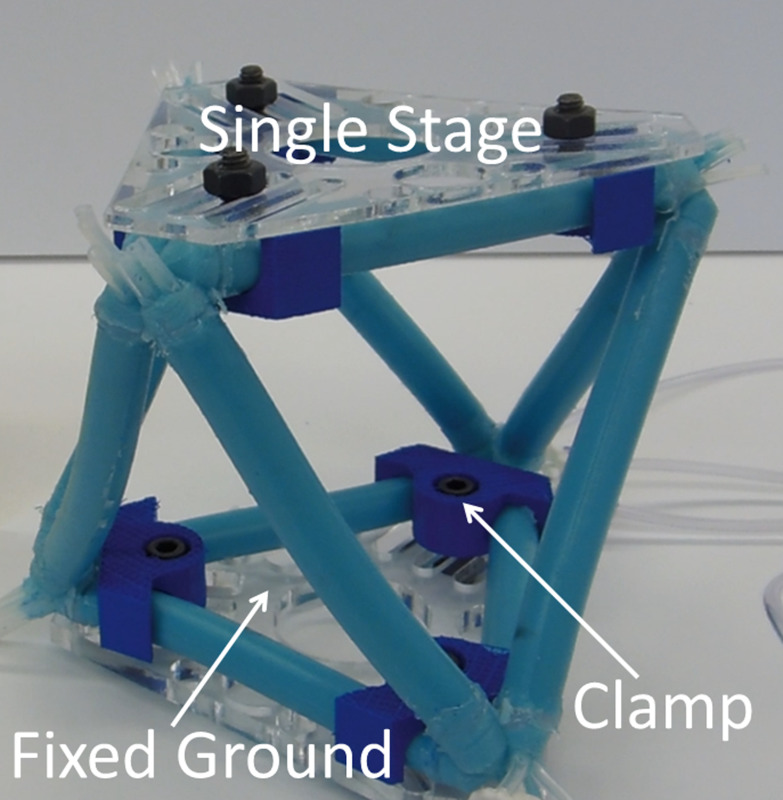
\includegraphics[width=.8\textwidth]{../Notes/figures/soft_parallel.jpg} 
			\end{tcolorbox} 
		\end{column}	
	\end{columns}
	\centering \footnotesize{A soft 6-6 Stewart manipulator. Jonathan Hopkins, 2015.}
\end{frame}


